% ============================================================================
% appendices.tex — References + Terminology + Appendix covers with full content
% Restructured 2026-03-17
% ============================================================================

% =============================================================================
% APPENDIX DIVIDER — full-bleed with Front Page image
% =============================================================================
\fullbleedpage
  {Appendices}

  {images/Front_Page.jpeg}

% =============================================================================
% APPENDIX OVERVIEW
% =============================================================================
% =============================================================================
% APPENDIX OVERVIEW — Single-page navigation
% =============================================================================
\clearpage
\begin{center}
{\Large\bfseries Appendix Overview}
\end{center}
\addcontentsline{toc}{section}{Appendix Overview}
\vspace{0.3cm}
{\small
\renewcommand{\arraystretch}{1.15}
\begin{tabular}{@{}p{1cm} p{2.5cm} >{\raggedright\arraybackslash}p{10cm}@{}}
\toprule
\multicolumn{3}{@{}l@{}}{\textbf{References} \hfill \textit{253 entries}} \\
\midrule
 & Bibliography & Full reference list in APA format \\
\midrule
\multicolumn{3}{@{}l@{}}{\textbf{Terminology} \hfill \textit{Key definitions}} \\
\midrule
 & Glossary & Abbreviations, risk channels, scenario labels, financial metrics \\
\midrule
\multicolumn{3}{@{}l@{}}{\textbf{Appendix A --- Complete ClimVaR Methodology} \hfill \textit{13 sections}} \\
\midrule
A.1--4 & Foundations & Notation, financial concepts, climate risk taxonomy, MRIOT framework \\
A.5 & ClimVaR model & Entity, company, portfolio, site, product-level formulas \\
A.6--7 & Loss terms & Physical ($\beta$, $\delta$, $\xi$, $\gamma$ + Shapley), Transition (CC), Nature ($\rho$) \\
A.8 & Scenarios & Physical $\times$ transition, intra-scenario uncertainty, Expected Shortfall \\
A.9 & Adaptation & Formal treatment of adaptation within the framework \\
A.10--13 & Extensions & Reputation/litigation risk, spatial estimation, ES derivation \\
\midrule
\multicolumn{3}{@{}l@{}}{\textbf{Appendix B --- Data and Hypotheses} \hfill \textit{7 sections}} \\
\midrule
B.1 & Model architecture & 17 input components, version history, data flow \\
B.2 & Facility database & 8{,}572 installed + 2{,}939 prospective; 120 countries; 64 attributes \\
B.3 & Financial calibration & 29 parameters, asset valuation matrices, 20 markets \\
B.4 & Physical risk data & CMIP at facility coordinates; 4 variables; 5 hazard types; $\sim$50M obs \\
B.5 & Supply chain & OECD MRIOT (75 countries $\times$ 45 sectors); 8 components \\
B.6 & Output structure & Aggregate (288$\times$14), annual (288$\times$305), sites (72$\times$592) \\
B.7 & Confidence & 48\% high / 34\% mixed / 17\% expert; sensitivity bounds \\
\midrule
\multicolumn{3}{@{}l@{}}{\textbf{Appendix C --- Scenario Trajectories} \hfill \textit{4 sections}} \\
\midrule
C.1 & Efficiency & PPA factor, PUE, carbon ratio trajectories by region (2024--2050) \\
C.2 & Carbon prices & BAU and NZT by region (\$/tCO$_2$, 2025--2050) \\
C.3 & Adaptation & Reduction rates by channel, strategy definitions \\
C.4 & Risk modeling & Cross-reference to A.6--A.9 \\
\midrule
\multicolumn{3}{@{}l@{}}{\textbf{Appendix D --- Systematic Literature Review} \hfill \textit{3 sections}} \\
\midrule
D.1 & Search strategy & Semantic search + structured screening across three research questions \\
D.2 & Results & Physical risk (Q1), insurance (Q2), valuation frameworks (Q3) \\
D.3 & Gap analysis & Coverage mapping against 9 dimensions; three structural gaps \\
\bottomrule
\end{tabular}
}

% =============================================================================
% REFERENCES (bibtex)
% =============================================================================
\clearpage
\thispagestyle{chapterstart}

\begingroup
\fontsize{11}{14}\selectfont
\setlength{\bibsep}{8pt plus 2pt minus 1pt}
\bibliographystyle{apalike}
\bibliography{references}
\endgroup

% =============================================================================
% TERMINOLOGY
% =============================================================================
% =============================================================================
% TERMINOLOGY — Symbols, Acronyms, and Key Definitions
% Placed after References, before Appendices
% =============================================================================

\clearpage
\section*{Terminology}
\addcontentsline{toc}{section}{Terminology}

\subsection*{Acronyms}

\begin{tabular}{@{}p{3cm}p{11cm}@{}}
APMEA & Asia-Pacific, Middle East, and Africa \\
AWB & Abundance Without Boundaries (AI growth scenario) \\
BAU & Business as Usual \\
BESS & Battery Energy Storage System \\
BI & Business Interruption \\
CAPEX & Capital Expenditures \\
CC & Carbon Cost (Scopes 1, 2, 3) \\
CDD & Cooling Degree Days \\
ClimVaR & Climate Value at Risk \\
CMIP6 & Coupled Model Intercomparison Project Phase 6 \\
COGS & Cost of Goods Sold \\
CSRD & Corporate Sustainability Reporting Directive (EU) \\
DC & Data Center \\
DCF & Discounted Cash Flow \\
ERCOT & Electric Reliability Council of Texas \\
ETS & Emissions Trading System \\
EV & Enterprise Value \\
GW & Gigawatt \\
I-O & Input-Output (Leontief analysis) \\
IEA & International Energy Agency \\
LTG & Limits to Growth (AI growth scenario) \\
MACC & Marginal Abatement Cost Curve \\
MRIOT & Multi-Regional Input-Output Tables \\
MW & Megawatt \\
NERC & North American Electric Reliability Corporation \\
NGFS & Network for Greening the Financial System \\
NPV & Net Present Value \\
NZT & Net Zero Transition \\
OPEX & Operating Expenses \\
PJM & PJM Interconnection (US Mid-Atlantic grid operator) \\
PPA & Power Purchase Agreement \\
PUE & Power Usage Effectiveness \\
RCP & Representative Concentration Pathway \\
SAI & Sustainable AI (AI growth scenario) \\
SLA & Service Level Agreement \\
TCFD & Task Force on Climate-related Financial Disclosures \\
UPS & Uninterruptible Power Supply \\
WACC & Weighted Average Cost of Capital \\
\end{tabular}

\subsection*{Channel Symbols}

\begin{tabular}{@{}p{3cm}p{11cm}@{}}
$\gamma$ & Cooling cost channel --- increased energy consumption from rising temperatures \\
CC$^{1,2,3}$ & Carbon cost channels --- Scope 1 (direct), Scope 2 (purchased electricity), Scope 3 (supply chain) \\
$\beta$ & Business interruption channel --- operational downtime from extreme events and grid failures \\
$\delta$ & Physical damage channel --- structural damage from acute events (floods, storms, seismic) \\
$\xi$ & Heat productivity channel --- outdoor labor efficiency loss from sustained heat exposure \\
$\sigma$ & Customer shift channel --- revenue loss from customer migration to lower-carbon providers \\
$\rho$ & Nature capital channel --- revenue loss from ecosystem degradation (water stress, biodiversity) \\
\end{tabular}

\subsection*{Financial Notation}

\begin{tabular}{@{}p{3cm}p{11cm}@{}}
$V_0$ & Baseline enterprise value (DCF, no climate adjustment) \\
$V^{cc}$ & Climate-adjusted enterprise value \\
ClimVaR & $V_0 - V^{cc}$ --- present value of climate-induced value erosion \\
ClimVaR\% & ClimVaR / $V_0$ --- climate risk intensity as percentage of enterprise value \\
$FCF^{(t)}$ & Free cash flow in year $t$ \\
$\omega$ & Weighted average cost of capital (WACC) \\
$\tau$ & Corporate tax rate \\
$T$ & Explicit forecast horizon (terminal year) \\
$AV$ & Asset value (book value of physical infrastructure) \\
\end{tabular}

\subsection*{Scenario Notation}

\begin{tabular}{@{}p{3cm}p{11cm}@{}}
RCP 2.6 / 4.5 / 8.5 & Physical climate pathways (Paris-aligned / moderate / high emissions) \\
BAU / NZT & Transition policy pathways (current policies / Net Zero by 2050) \\
LTG / SAI / AWB & AI growth scenarios (constrained / sustainable / unconstrained) \\
Baseline / Selective / Proactive & Adaptation strategies (no action / new builds only / full portfolio) \\
Q25 / MEAN / Q95 & Statistical reporting quantiles within each scenario \\
\end{tabular}

\subsection*{Key Definitions}

\begin{tabular}{@{}p{3cm}p{11cm}@{}}
Installed base & 8{,}572 operational data center facilities (90.8~GW), pre-2025 \\
Prospective & AI-era facilities planned or projected through 2050 (615--2{,}939 depending on scenario) \\
Adaptation wedge & Difference in ClimVaR between Baseline and Proactive strategies \\
Residual risk & ClimVaR remaining after Proactive adaptation (61\% of total on installed base) \\
Channel fingerprint & The distinctive risk channel composition of a region or facility \\
Shapley value & Fair attribution of aggregate risk to individual contributing hazards \\
Leontief inverse & $(I - DA^T)^{-1}$ --- captures direct and indirect supply chain propagation \\
Pass-through rate & Fraction of upstream disruption transmitted to downstream operations \\
\end{tabular}

\appendix

% =============================================================================
% APPENDIX A — Shapley (Complete ClimVaR Methodology)
% =============================================================================
\clearpage\thispagestyle{chapterstart}

\begin{center}
\begin{tikzpicture}
  \clip (0,0) circle (3cm);
  \node[inner sep=0pt] at (0,0) {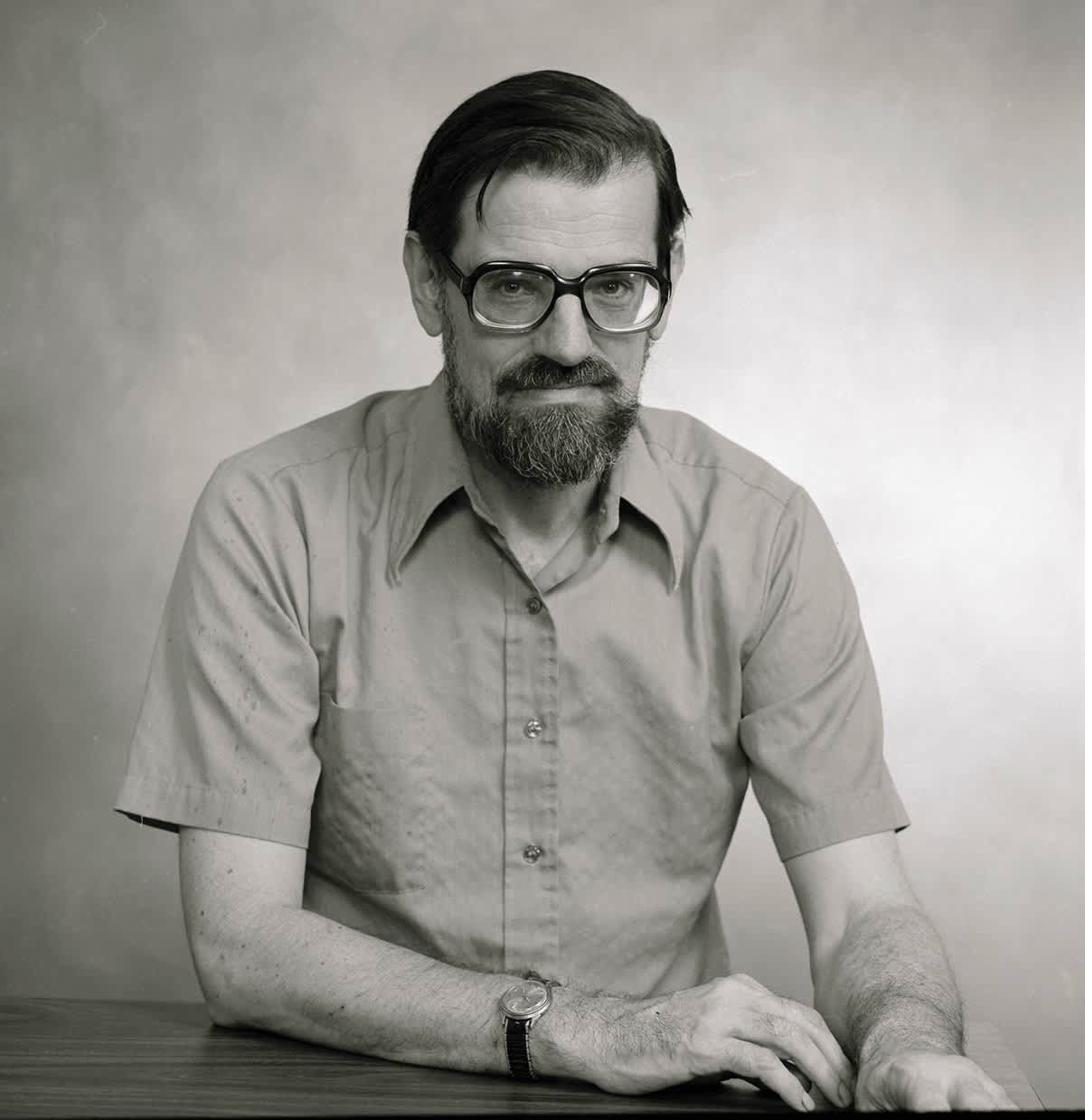
\includegraphics[width=6cm]{images/SHAPLEY}};
\end{tikzpicture}
\end{center}

\vspace{4mm}

\begin{center}
{\displayfont\fontsize{24}{28}\selectfont\color{SEGreen}Appendix A\par}
\vspace{2mm}
{\displayfont\fontsize{18}{22}\selectfont\color{SESubtitle}Complete ClimVaR Methodology\par}
\vspace{2mm}
{\fontsize{9}{11}\selectfont\color{SESubtitle}Lloyd Shapley (1923--2016)\par}
\end{center}

\vspace{4mm}

\begin{pullquote}
Each player receives a payoff equal to his average marginal contribution over all possible orderings of the players.
\end{pullquote}

\vspace{4mm}

\begin{twocolbody}
\noindent Climate risk for data centers is not a single hazard---it is a portfolio of five interacting channels. Because these channels interact non-additively (cooling stress amplifies business interruption; carbon pricing compounds with physical damage), simple summation double-counts risk.

The Shapley value from cooperative game theory provides a principled decomposition. For $n=5$ risk channels, it evaluates all $2^5 = 32$ coalition combinations per facility, attributing each channel's marginal contribution to total ClimVaR. The decomposition satisfies efficiency, symmetry, and the null player property.

\subsubsection*{Contents}
\begin{itemize}[leftmargin=10pt, itemsep=2pt]
  \item A.1 Complete ClimVaR methodology (Epelbaum 2025)
  \item A.2 Shapley value formulation for risk attribution
  \item A.3 Computational implementation (32 coalitions)
  \item A.4 Expected Shortfall estimation
\end{itemize}
\end{twocolbody}

% --- Full ClimVaR methodology from Thomas ---
\clearpage
% =============================================================================
% APPENDIX B: COMPLETE ClimVaR METHODOLOGY
% Based on Epelbaum (2025). Trimmed for whitepaper: full derivations
% deferred to the original reference.
% =============================================================================
\newpage
\section{ClimVaR Methodology} \label{sec:climvar-full}

% Color definitions needed for figures in this appendix
\definecolor{BLUE_MAIN}{RGB}{0, 102, 161}
\definecolor{BLUE_PASTEL}{RGB}{55,127,171}
\definecolor{RED_MAIN}{RGB}{227, 114, 88}
\definecolor{RED_PASTEL}{RGB}{164,98,76}
\definecolor{RED_PASTEL_2}{RGB}{231, 143, 115}
\definecolor{RED_DARK}{RGB}{196,172,107}
\definecolor{GREEN_MAIN}{RGB}{146, 178, 119}
\definecolor{GREEN_DARK}{RGB}{109, 142, 81}
\definecolor{GREEN_DARKER}{RGB}{73, 95, 54}
\definecolor{GREEN_REL}{RGB}{64, 130, 109}
\definecolor{BROWN_MAIN}{RGB}{194, 144, 124}
\definecolor{BROWN_DARK}{RGB}{163, 98, 84}
\definecolor{GOLD_MAIN}{RGB}{238, 232, 170}
\definecolor{GOLD_DARK}{RGB}{255, 219, 88}

% Macro definitions for Expected Shortfall plots
% fillbetween library loaded in preamble
\def\oe9{1e9}
\def\sig1{sqrt(0.2)*\oe9}
\def\sig2{sqrt(0.1)*\oe9}
\def\sig3{sqrt(0.3)*\oe9}
\def\muC{2}
\def\sigC{sqrt(0.5)*\muC}
\def\sigLsq{ (\sigC/\muC)^2 + ((\sig1+\sig2+\sig3)/\oe9)^2 + (\sigC/\muC)^2*((\sig1+\sig2+\sig3)/\oe9)^2 }
\def\muL{\muC*\oe9}
\def\muLlog{ln(\muL/sqrt(1+\sigLsq))}
\def\sigL{sqrt(ln(1+\sigLsq))}
\def\sigD{sqrt( (\sig1+\sig2+\sig3)^2 )}
\def\sigDcv{ \sigD/\oe9 }
\def\muDlog{ln(\oe9/sqrt(1+\sigDcv^2))}
\def\sigS3sq{ (\sigC/\muC)^2 + ((\sig1+\sig2)/\oe9)^2 + (\sigC/\muC)^2*((\sig1+\sig2)/\oe9)^2 }
\def\muS3log{ln(\muL/sqrt(1+\sigS3sq))}
\def\sigS3{sqrt(ln(1+\sigS3sq))}
\def\sigBothsq{ ((\sig1+\sig2)/\oe9)^2 }
\def\muBothlog{ln(\oe9/sqrt(1+\sigBothsq))}
\def\sigBoth{sqrt(ln(1+\sigBothsq))}

\tikzset{
    declare function={
        norminv(\p)=sqrt(-2*ln(1-\p))-(2.515517+0.802853*sqrt(-2*ln(1-\p))+0.010328*(-2*ln(1-\p)))/(1+1.432788*sqrt(-2*ln(1-\p))+(0.189269+0.001308*sqrt(-2*ln(1-\p)))*sqrt(-2*ln(1-\p)))*sqrt(-2*ln(1-\p));
        normcdf(\x)=1/(1+exp(-1.6545*\x*(1+0.25*\x)));
    }
}
% \CDF operator not needed — "CDF" used as plain text

\subsection{Introduction} \label{sec:intro}

Climate change is one of the central problem humanity has to tackle in the 21st century. The frequency of extreme climate events is already increasing, and this tendency can only worsen if no action is taken to limit anthropic carbon emissions. In recent years, several climate/financial regulation frameworks \cite{EUC}-\cite{Deloitte} were developed, aiming at collecting climate related data and be somewhat prescriptive \cite{EuropeanClimateLaw} on how to decarbonate. Nevertheless, the current accounting norms (GAAP, IFRS...) do not even fully capture simple materiality aspects, making relevant financial decisions at public and private level difficult.

\vspace{0.2cm}

As we will see in section \ref{sec:related}, several studies have been done in the past years on the financial impact  caused by some climate risks. But most of these studies focus on one aspect of the problem: a specific transition risk \cite{Transition1} like carbon cost \cite{Adenot}\cite{RoncalliCC} or litigation \cite{Litigation1}\cite{Litigation2}, nature risk \cite{NatureF1}\cite{NatureF2}\cite{NatureF3}\cite{RoncallliBiodivBook}\cite{RoncalliNatureCap}, or physical climate risk \cite{LeGuenedal}. 


\vspace{0.2cm}

A unifying approach is therefore somewhat lacking, though most of the tools needed to get there have already been developed. 

\vspace{0.2cm}

In this paper we will use a standard Discounted Cash Flow (DCF) approach to cover all the major climate risks to be faced in the years/decades to come.

\vspace{0.2cm}

Our aim is to help public and private organisms measure the economic viability of systems. Five types of systems will be studied: 
\begin{itemize}
\item[•] A portfolio of financial products.
\item[•] A company.
\item[•] An entity within a company.
\item[•] A site of an entity\footnote{We consider in all the following an entity to be a company part belonging to a specific country and operating within a specific sector of activity.}.
\item[•] A company product (depending on several sites). A product is produced on several sites, and one site can produce several products.
\end{itemize}

\vspace{0.2cm}

Having access to better financial assessments of systems should allow for a better resilience of the economic actors with respect to climate change, and should ease the transformations needed to fight it: decarbonate the supply chain, build floodgates, avoid brown sectors when it makes sense...

\vspace{0.2cm}

Our objective will be reached if regulators, auditors, public and private actors can start using the white box formalism that we (though obviously building a lot on existing works) develop in the next sections. This should help them really assess the economic profitability of the projects/systems they supervize by duly accounting for climate change.

\vspace{0.2cm}

As already stated, we will adapt a standard DCF approach to estimate the future valuation $V$ of a system. In all the following, the system can be one of the fives already stated. We will augment the traditional DCF approach by considering variations related to climate. These variations can be related to 
\begin{itemize}
\item[$\bullet$] physical risk: flood, drought, wildfire \cite{IPPC1}\cite{IPPC2}...
\item[$\bullet$] transition risk: carbon tax, customer shift  \cite{Adenot}\cite{RoncalliCC}\cite{Bouchet}\cite{NGFS1}..
\item[$\bullet$] nature risk: loss of nature capital \cite{RoncalliNatureCap}
\end{itemize}

We call our central DCF formula embedding climate risks ClimVaR (for Climate Value at Risk)

\vspace{0.2cm}

The rest of this note is devoted to deriving ClimVaR for the five systems already mentioned.  It is organized as follows. Section~\ref{sec:related} discusses related work, insisting on the fact that the current paper builds on existing (but siloed) studies. Section~\ref{sec:notation} regroups all notations. The tools developed in this paper are not advanced, but put together they cover a large range of concepts. The reader should therefore refer to this section to understand the approach and all symbols. Section~\ref{sec:climvar} presents the central result of this work: a valuation formula encompassing physical and transition climate-related effects. Section~\ref{sec:climvar-terms} summarizes the derivation of individual loss terms, referring the reader to \citet{epelbaum2025} for the complete mathematical treatment. Section~\ref{sec:scenario} elaborates on the scenario and uncertainty topic. The link with the usual Value At Risk (VaR) is also made. The financially knowledgeable reader pondering on the use of the ClimVaR term will benefit from \ref{sec:shortfall}. Adaptation strategies and their economic merit are discussed in the main text (Chapter~III, Finding~4). Extensions to additional transition risks (reputation, litigation, technology, investor sentiment) are deferred to subsequent work.


\subsection{Related work} \label{sec:related}

Relating climate risks to financial impacts is not a new topic, but it has seen a rise of interest in recent years.

\vspace{0.2cm}

The climate/economy relationship could be traced back to the Meadows Report \cite{Meadows1972}, which initiated the works on Integrated assessment Models (IAMs), coupling classical macro-economic equations with exogenous (climate, but not only) economic data. Following its steps, numerous IAMs \cite{DICE}\cite{GLOBIOM}\cite{Remind}\cite{MESSAGE} were developed in the past 50 years, adding among other things local (by opposition to world or large regions) and sectoral modelling.

\vspace{0.2cm}

Climate risks could loosely be divided into 3 different categories:
\begin{itemize}
\item[•] Physical risk \cite{IPCCRisk} correspond to the impact of climate events on human activity: a strong wind damaging a building, a flood interrupting business activities...  Several papers \cite{LeGuenedal}\cite{BID}\cite{Bernhofen}\cite{Azzone} have investigated the impact of these physical events onto financial activities.
\item[•] Nature (biodiversity) risk is a more recent center of interest. It analyzes the effect of nature/ecosystem/biosphere degradation onto economic activities \cite{RoncalliNatureCap}\cite{SPGNatureBio}\cite{NatureF4}. As we are approaching several planetary limits \cite{PlanetaryBoundaries}\cite{PlanetaryBoundariesUpdate}, this topic should see intense activities in the years to come.
\item[•] Transition risk represents the human adaptation to climate change, in the forms of laws, norms, bans, taxes, individual consumer behaviours... It may be the topic that have been the focus of the most attention in the past decade \cite{RoncalliCC}\cite{TransitionRiskCaldecott}\cite{FDIC}\cite{TCFD}, but recent changes in international geopolitics \cite{OmnibusRollback} could make this risk less pregnant than the physical one in the years to come.
\end{itemize}

Some paper on Climate Value At Risk \cite{RoncalliVaR}\cite{MSCIClimateVaR} already exist, but they do not yet offer a unifying, quantitative, white box analysis encompassing all the risks previously mentionned. The present work aims to do just so.

\subsection{Notation} \label{sec:notation}

\subsubsection{Generic concepts}

\begin{itemize}
\item[•] $t$: times. In the present paper year is the time unit, unless specified otherwise.
\item[•] $\nu$: Scenario (more on scenarios in section \ref{sec:scenario-inter})
\item[•] $\lambda$: Intra scenario uncertainty (more on it and link with VaR in section \ref{sec:scenario-intra}).
\item[•] $r$: Supply chain rank. $0$ means direct operation (i.e. a system direcly operated by the project leader). $1$ means direct supplier (meaning supplier to which the project leader directly buys). $1+$ means all suppliers (direct and indirect. Indirect suppliers are suppliers of suppliers, suppliers of suppliers of suppliers... And so on). $0+$ means all contributions, direct and suppliers.
\end{itemize}

\subsubsection{Company related concepts}

We will denote
\begin{itemize}
\item[•] $FP$: Financial Portfolio.
\item[•] $C$: Company (possibly part of for a financial portfolio).
\item[•] $E$: Entity of a company.
\item[•] $S$: Site of an entity. We will interchangeably use assets $a$.
\item[•] $P$: Product.
\item[•] $c$: World countries.
\item[•] $s$: Activity sectors. we take the ISIC standard \cite{ISIC} for encoding the activity sectors, and consider the 45 ISIC sectors used in the 2023 OECD work \cite{OECD1}\cite{OECD2} unless stated otherwise.
\item[•] $S^{(1)}$: Carbon equivalent emissions  within a year corresponding to direct system actitivities, called Scope 1 \cite{S1} in the litterature.
\item[•] $S^{(2)}$: Carbon equivalent emissions within a year corresponding to system electricity consumptions, called Scope 2 \cite{S2} in the litterature.
\end{itemize}


\subsubsection{Financial concepts}

We will note

\begin{itemize}
\item[•] $V$: Valuation.  
\item[•] $\text{VaR}$: Valuation At Risk.
\item[•] $FCF$: Future Cash Flow. .
\item[•] $T$: Terminal time value.
\item[•] $g$: Perpetual growth rate.
\item[•] $g^{(t)}$: Yearly growth rate.
\item[•] $Y$: System gross revenues. 
\item[•] $\omega$ (or $W\!ACC$): Weighted Average Cost of Capital. $\omega$ will be preferred in equations. $W\!ACC$ variation is deferred to future work.
\item[•] $DCF$: Discounted Cash Flow. $DCF^{(t)}=FCF^{(t)}/\left(1+\omega\right)^t$. 
\item[•] $COGS$: Cost Of Goods Sold.
\item[•] $c$: $COGS$ to Revenue ratio.
\item[•] $OPEX$: Operating Expenses.
\item[•] $o$: $OPEX$ to Revenue ratio.
\item[•] $s$: Salary to Revenue ratio. 
\item[•] $P$: Absolute (monetary) system purchases will be noted as $P$.
\item[•] $p$: system purchases ratio will be noted as $p$, and we consider $p=c-s$. 
\item[•] $so$: Outdoor salary mass to Revenue ratio.
\item[•] $si$: Indoor salary mass is not used in the present analysis. Obviously $s=si+so$.
\item[•] $e$: Electricity expenses to Revenue ratio.
\item[•] $ec$: Electricity cooling expenses to Revenue ratio.
\item[•] $\tau$: system (federal) tax rate.
\item[•] $CFO$: Cash Flow from Operation.
\item[•] $CAPEX$: CAPital EXpenditures.
\item[•] $NWC$: for Net Working of Capital. 
\item[•] $DA$: for Depreciation (and Amortization)\footnote{In our approach we follow the Generally Accepted Accounting Principles (GAAP)\cite{KPMG}, which are for instance somewhat different from the French accounting formalism.}. 
\item[•] $k$: for $CAPEX$ over Revenue ratio. 
\item[•] $n$: for $NWC$ over Revenue ratio. 
\item[•] $d$: for $DA$ over Revenue ratio. 
\item[•] $op$: Operating Profit over Revenue Ratio. $op=1-c-o$.
\item[•] $i$: Insurance premium.
\item[•] $AV$: Asset Value (in the sense of hard assets: buildings...).
\end{itemize}

\subsubsection{Climate risk related concepts}

\begin{itemize}
\item[•] $cc$: Climate change (by contrast with quantities computed without considering it).
\item[•] $h$: Climate hazard (drought, flood, wild fire...).
\item[•] $\sigma$: Customer shift.
\item[•] $\beta$:  Business Interruption Days (BID) (as a fraction of year) at country sector level.
\item[•] $\chi$:  Business Interruption Days (BID) at asset site level.
\item[•] $\rho$: Degradation of renewable nature capital (as a \% of revenue).
\item[•] $\delta$: Damages on assets (as a \% of asset value).
\item[•] $CC^{(i)}$: Carbon costs related to scope $i$.
\item[•] $\xi$: Heat Productivity Loss \cite{HI1}\cite{HI2}\cite{HPL1}\cite{HPL2}\cite{HPL3}.
\item[•] $\gamma$: Cooling cost increase \cite{CDD} (from a reference to a future time period).
\end{itemize}

\subsubsection{Multi Regional Input Output table (MRIOT) related concepts}

MRIOT is a rich topic on its own, that we only minimally cover in this paper to the extent of our need.

\begin{itemize}
\item[•] $Z_{_{cs,c's'}}$: Multi Regional Input Ouput Table (MRIOT). Following \cite{MillerMRIOT}, we adopt the convention where rows of $Z$ correspond to suppliers and columns to clients. $Z_{_{cs,c's'}}$ is therefore a financial flux within a year\footnote{Usually in USD or M~USD.} between sector $s'$ of country $c'$, buying goods from  sector $s$ of country $c$.
\item[•] $X_{_{cs}}$: Total financial output of sector $s$ of country $c$. 
\item[•] $A_{_{cs,c's'}}$:  $A$ Technical coefficient matrix. Coefficients as $A_{_{cs,c's'}}=Z_{_{cs,c's'}}/X_{_{c's'}}$.

\item[•] $L_{_{cs,c's'}}$:  Leontief matrix. $L=\mathbb{I}+ A^T+\left(A^T\right)^2+\cdots= \left(\mathbb{I}-A^T\right)^{-1}$.
\end{itemize}

\subsubsection{Carbon cost related concepts}

We will use the following notations

\begin{itemize}
\item[$\bullet$] $C^{(t)}_{_c}$: "Raw" carbon price (as USD per tons of CO2 equivalent emissions, or TCO2e). Carbon prices \cite{WorldBankCC} are given at country level and are considered time dependent.
\item[$\bullet$] $F^{(t)}_{_s}$: Free allocation rates. These are sectoral allocations that allow sectors to discount part of their carbon costs. In our approach, Free allocations are always present in Business as Usual scenarios and removed after 2030 for other ones. More on scenarios in section \ref{sec:scenario}.
\item[$\bullet$] Passthrough $P_{_s}$ at sector level. Considered to be $1$ for the remaining of this paper. This is a strong assumption that we will relax in future studies.
\item[$\bullet$] $\mathcal{C}^{(t)}_{_{cs}}$: Combined "Raw" carbon price. $\mathcal{C}^{(t)}_{_{cs}}=F^{(t)}_{_s}C^{(t)}_{_c}P_{_s}=F^{(t)}_{_s}C^{(t)}_{_c}$.
\item[$\bullet$] $I^{(i)}_{_{cs}}$: Carbon intensities (TCO2e per revenue (USD)) for scope $i$. When $i$ is unspecified, it is for scope 1. These country sector intensities can be evaluated in several manners: having access to database of company emissions + financial data \cite{CDP}, or a MRIOT approach (like the one performed by Exiobase \cite{Exiobase})...
\end{itemize}

\subsection{ClimVaR model} \label{sec:climvar}

We leave aside the notion of scenario and uncertainty for the time being. We will come back on these important topics in section \ref{sec:scenario}. As is standard in valuation approaches, ClimVaR will take major financial information from income statements, balance sheets and cash flows to form the Discounted Cash Flow. ClimVaR novelty resides in how it computes and aggregates climate risk effects on different parts of the Discounted Cash Flow. As stated in section \ref{sec:intro}, we want to derive these effects for five systems (from the finer to the coarser level): products, sites, entities, companies, financial portfolios. As we will see in the following, financial portfolios can be seen as the aggregation of company valuation computations, and the same goes for entities with respect to companies and sites with respect to entities. The relation is not one to many but many to many for products to sites valuation: a product is generally produced by several sites, but sites usually also produce parts of several products at once.

\vspace{0.2cm}

We will start with the entity computation, that is the simpler to explain on its own. From it we will trivially derive ClimVaR formulas for companies and financial portfolios. We will then explain the adaptations needed on the entity formula to get the sites and finally the product ones.

\subsubsection{Entity ClimVaR} \label{sec:climvar-entity}

\vspace{0.2cm}

A DCF model \cite{Kruschwitz}\cite{Valuation} estimates the current value (at current time $0$) of a system as the sum of it's future Discounted Cash Flows. We first focus our attention on an entity, belonging to a sector $s$ of a country $c$. Valuation reads there

\begin{align}
V^{(E)}_{_{cs}}&=\sum_{t=1}^{+\infty}\frac{FCF^{(t)}_{_{cs}}}{(1+WACC_{_{cs}})^t}\;,\label{eq:base-val}
\end{align}

where $W\!ACC$ is assumed to be time/climate independant and equal to $\omega_{_{cs}}$. 

\vspace{0.2cm}

It is good practice to take a terminal value year $T$ (which we consider constant at company level), after which the system is experiencing fixed perpetual growth (Gordon Growth Model) $g_{_{cs}}$. 

\begin{align}
V^{(E)}_{_{cs}}&=\sum_{t=1}^{T}\frac{FCF^{(t)}_{_{cs}}}{\left(1+\omega_{_{cs}}\right)^t}
%
+\frac{FCF^{(T)}_{_{cs}}}{\left(1+\omega_{_{cs}}\right)^t}\frac{1+g}{\omega_{_{cs}}-g_{_{cs}}}\;.
\end{align}
To simplify the notation, we will take 
\begin{align}
FCF^{(T+1)}_{_{cs}}&=FCF^{(T)}_{_{cs}}\frac{(1+g_{_{cs}})(1+\omega_{_{cs}})}{(\omega_{_{cs}}-g_{_{cs}})}\;,\label{eq:perpetfcf}
\end{align}
so that
\begin{align}
V^{(E)}_{_{cs}}&=\sum_{t=1}^{T+1}\frac{FCF^{(t)}_{_{cs}}}{\left(1+\omega_{_{cs}}\right)^t}\;.
\end{align}

\vspace{0.2cm}

In our model, we will be interested by the Climate Value at Risk (ClimVaR) \cite{Kruschwitz}\cite{Valuation}\cite{Damodaran1}: namely the difference between a valuation without and with climate change. This is the central quantity that we want to estimate

\begin{align}
\text{VaR}^{(E)}_{_{cs}}&=\Delta V^{(E)}_{_{cs}}=V^{(E)}_{_{cs}}-V^{(E,cc)}_{_{cs}}
%
=\sum_{t=1}^{T+1}\frac{FCF^{(t)}_{_{cs}}-FCF^{(t,cc)}_{_{cs}}}{\left(1+\omega_{_{cs}}\right)^t}\;.\label{eq:var}
\end{align}

To be noted, we will also be interested by a $\delta$VAR, namely

\begin{align}
\delta \text{VaR}^{(E)}_{_{cs}}&=\frac{\Delta V^{(E)}_{_{cs}}}{V^{(E)}_{_{cs}}}\;,\label{eq:delta-var}
\end{align}

that estimates the share of the total value at risk\footnote{Keep in mind that the climate can generate value, in the case of customer shift for instance.}.

\vspace{0.2cm}

The FCF at time $t$ reads \cite{Damodaran1}

\begin{align}
FCF^{(t)}_{_{cs}}&=CFO^{(t)}_{_{cs}}- CAPEX^{(t)}_{_{cs}} - \delta NWC^{(t)}_{_{cs}}\;,
\end{align}


In a first approach, we will assume that both $NWC$ (corresponding to short term assets and liabilities cash fluxes) and $CAPEX$ do not depend on climate change (as we will see, we will consider fixed assets accelerated degradation because of climate change via the OPEX term in CFO. To be noted $CAPEX$ will play a role when taking into account climate actions), and that they represent a constant fraction of revenues $Y$:

\begin{align}
\delta NWC^{(t)}_{_{cs}}&=
%
NWC^{(t)}_{_{cs}}- NWC^{(t-1)}_{_{cs}}\approx
%
 n_{_{cs}}\left(Y^{(t)}_{_{cs}} - Y^{(t-1)}_{_{cs}}\right)\;,\notag\\
%
CAPEX^{(t)}_{_{cs}} & \approx k_{_{cs}}Y_{_t}\;.
\end{align}

In that case

\begin{align}
\text{VaR}^{(E)}_{_{cs}}&=\sum_{t=t_0+1}^{T+1}\frac{CFO^{(t)}_{_{cs}}-CFO^{(t,cc)}_{_{cs}}}{(1+w)^t}\;.
\end{align}

$CFO$ reads

\begin{align}
CFO^{(t)}_{_{cs}}&=NOPAT^{(t)}_{_{cs}}+DA^{(t)}_{_{cs}}\notag\\
%
&=\left[Y^{(t)}_{_{cs}}-COGS^{(t)}_{_{cs}}-OPEX^{(t)}_{_{cs}}-DA^{(t)}_{_{cs}}\right]
%
\left[1-Tax^{(t)}_{_{cs}}\right]+DA^{(t)}_{_{cs}}\;,
\end{align}

In our model, we assume that taxes are not affected by climate change\footnote{We will see later that Carbon Taxes are taken into account via the Revenue and the OPEX channel} and are constant ($\tau_{_{cs}}$) through time. In addition, we also assume that $DA$ is not affected by climate change (again, additional costs incured to repair buildings will be considered as OPEX) and is a constant share of the total revenue
\begin{align}
DA^{(t)}_{_{cs}}&\approx d_{_{cs}} Y^{(t)}_{_{cs}}\;.
\end{align}

We therefore focus our attention on the Operating profit

\begin{align}
OP^{(t)}_{_{cs}}&=Y^{(t)}_{_{cs}}-COGS^{(t)}_{_{cs}}-OPEX^{(t)}_{_{cs}}\;.\label{eq:profit}
\end{align}

And our central climate VAR (\ref{eq:var}) becomes
\begin{align}
\text{VaR}^{(E)}_{_{cs}}&=
%
\sum_{t=1}^{T+1}\frac{1-\tau_{_{cs}}}{\left(1+\omega_{_{cs}}\right)^t}\left[OP^{(t)}_{_{cs}}-OP^{(t,cc)}_{_{cs}}\right]\notag\\
%
&=\sum_{t=1}^{T+1}\frac{1-\tau_{_{cs}}}{\left(1+\omega_{_{cs}}\right)^t}\left[
%
Y^{(t)}_{_{cs}}-Y^{(t,cc)}_{_{cs}}-\left(COGS^{(t)}_{_{cs}}-COGS^{(t,cc)}_{_{cs}}\right)
%
\right.\notag\\
%
&\left.  -\left(OPEX^{(t)}_{_{cs}}-OPEX^{(t,cc)}_{_{cs}}\right)\right]\;.
\end{align}

We continue our modelling by assuming that $COGS$ and $OPEX$ are proportional to revenues \cite{Damodaran3}
\begin{align}
COGS^{(t)}_{_{cs}}&\approx c_{_{cs}} Y^{(t)}_{_{cs}}\;,&
%
OPEX^{(t)}_{_{cs}}&\approx o_{_{cs}} Y^{(t)}_{_{cs}}\notag\\
%
COGS^{(t,cc)}_{_{cs}}&\approx c^{(t,cc)}_{_{cs}} Y^{(t,cc)}_{_{cs}}\;,&
%
OPEX^{(t,cc)}_{_{cs}}&\approx o^{(t,cc)}_{_{cs}} Y^{(t,cc)}_{_{cs}}\;,
\end{align}
so that, recalling that
\begin{align}
op_{_{cs}}&=1- c_{_{cs}}-o_{_{cs}}\;,
\end{align}
we get
\begin{align}
\text{VaR}^{(E)}_{_{cs}}=\sum_{t=1}^{T+1}\frac{1-\tau_{_{cs}}}{\left(1+\omega_{_{cs}}\right)^t}&\left[
%
op_{_{cs}}\left(Y^{(t)}_{_{cs}}-Y^{(t,cc)}_{_{cs}}\right)\right.\notag\\
%
&\left. +\left(c^{(t,cc)}_{_{cs}}- c_{_{cs}}\right)Y^{(t,cc)}_{_{cs}}
%
+\left(o^{(t,cc)}_{_{cs}}- o_{_{cs}}\right)Y^{(t,cc)}_{_{cs}}
\right]\;.\label{eq:central}
\end{align}

Future system revenues will be taken with a time dependent cumulated growth rate $g^{(t)}_{_{cs}}$, so\footnote{In practice We will presumably have access to yearly growh rates $yg$, so
\begin{align*}
g^{(t)}_{_{cs}}&=\prod_{t'=1}^{t}\left(1+yg^{(t')}_{_{cs}}\right)-1
\end{align*}} 

\begin{align}
Y^{(t)}_{_{cs}}&=\left(1+g^{(t)}_{_{cs}}\right)Y_{_{cs}}\;,
\end{align}
with $Y_{_{cs}}$ the current (at present time) revenues. Our model thus has currently the following unknowns:
\begin{itemize}
\item[•] future revenues $Y^{(t,cc)}_{_{cs}}$ taking into account climate change
\item[•] future COGS to revenue ratio $c^{(t,cc)}_{_{cs}}$ taking into account climate change
\item[•] future OPEX to revenue ratio $o^{(t,cc)}_{_{cs}}$ taking into account climate change
\end{itemize}

It is time to explicit these terms and how climate risks contribute to them.

\paragraph{Revenue change caused by climate effects}

We will consider three climate change effects on revenues:
\begin{itemize}
\item[•] Customer shift (market transition risk) $\sigma^{(t)}_{_{cs}}$
\item[•] total Business Interruption Days (BID) $\beta^{(t)}_{_{cs}}$: from interruption within the entity and from its supply chain (physical risk).
\item[•] Loss of ecosytemic effect: degradation of renewable $\rho^{(t)}_{_{cs}}$ nature capital (nature risk). 
\end{itemize}
These terms are derived in detail in \citet{epelbaum2025}. We thus write
\begin{align}
Y^{(t,cc)}_{_{cs}}&=\left(1-\sigma^{(t)}_{_{cs}}\right)\left(1-\beta^{(t)}_{_{cs}}\right)
%
\left(1-\rho^{(t)}_{_{cs}}\right)Y^{(t)}_{_{cs}}\;,\label{eq:revenue-cc}
\end{align}

\paragraph{OPEX change caused by climate effects}

The only OPEX change we consider is related to damages on buildings. We take a simple model, where the insurance cost\cite{Cummins} is increased due to future expected damages on buildings
\begin{align}
o^{(t,cc)}_{_{cs}}Y^{(t,cc)}_{_{cs}}&=o_{_{cs}}Y^{(t,cc)}_{_{cs}}+\left(1+i_{_{cs}}\right) AV_{_{cs}} \delta^{(t)}_{_{cs}}\;,
\end{align}
where $AV_{_{cs}}$ is the total (hard) assets owned by entity $cs$, $i_{_{cs}}$ is an insurance premium and $\delta^{(t)}_{_{cs}}$ is the future damage fraction loss of the assets (see \citet{epelbaum2025} for the full derivation). In the future we will also make use of asset value to reference revenue ratio
\begin{align}
 av_{_{cs}}&=\frac{ AV_{_{cs}}}{ Y_{_{cs}}}
\end{align}

\paragraph{COGS change caused by climate effects}

We will consider three climate change effects on COGS: 
\begin{itemize}
\item[•] Carbon cost , both from direct $CC^{(t1)}$ and indirect emissions: supply chain, from scope 2 and scope 3 emissions. We will respectively consider $CC^{(t2)}$ and $CC^{(t3)}$ carbon costs (policy transition risk).
\item[•] Heat Productivity loss $\xi^{(t)}_{_{cs}}$ (physical risk).
\item[•] Cooling cost increase $\gamma^{(t)}_{_{cs}}$ (physical risk).
\end{itemize}

To be able to apply them, we will need two specific parts of the COGS to revenue ratio
\begin{itemize}
\item[•] outdoor salary mass to Revenue ratio $so$
\item[•] cooling costs to Revenue ratio $ec$
\end{itemize}
so that
\begin{align}
c^{(t,cc)}_{_{cs}}Y^{(t,cc)}_{_{cs}}&=c_{_{cs}}Y^{(t,cc)}_{_{cs}}+so_{_{cs}}\, \xi^{(t)}_{_{cs}} Y^{(t,cc)}_{_{cs}}+ ec_{_{cs}} \gamma^{(t)}_{_{cs}}Y^{(t,cc)}_{_{cs}}
%
+\sum_{i=1}^3CC^{(ti)}_{_{cs}}\;.
\end{align}

\paragraph{Combining all effects}

Taking into account the results of the three previous sections, our central equation becomes

\vspace{0.1cm}

\begin{tcolorbox}[colback=red!5!white,colframe=red!70!black,title=\textbf{ClimVaR central formula},halign title=flush center]
\begin{align}
\text{VaR}^{(E)}_{_{cs}}&=
%
\sum_{t=1}^{T+1}
%
\frac{\left( 1-\tau_{_{cs}}\right)}{\left(1+\omega_{_{cs}}\right)^t}
%
\left[op_{_{cs}}\left(Y^{(t)}_{_{cs}}-Y^{(t,cc)}_{_{cs}}\right)
%
+Y^{(t,cc)}_{_{cs}}\left(so_{_{cs}}\, \xi^{(t)}_{_{cs}} + ec_{_{cs}} \gamma^{(t)}_{_{cs}}\right)
%
\right.\notag\\
%
&\left. +\sum_{i=1}^3CC^{(ti)}_{_{cs}}+\left(1+i_{_{cs}}\right) AV_{_{cs}} \delta^{(t)}_{_{cs}}
%
\right]\;.\label{eq:central2}
\end{align}
\end{tcolorbox}

\vspace{0.1cm}

This is the central result of this work. The first term in the bracket corresponds to revenue loss, the last one to OPEX increase and the others to COGS increases. Let us recall that $T+1$ terms are the same than $T$ modulo the prefactor shown in (\ref{eq:perpetfcf}). Finally, since without climate change
\begin{align}
V^{(E)}_{_{cs}}&=\sum_{t=1}^{T+1}\frac{\left(1+g^{(t)}_{_{cs}}\right)Y_{_{cs}}}{\left(1+\omega_{_{cs}}\right)^t}
%
\left[op_{_{cs}}\left(1-\tau_{_{cs}}\right)+\tau_{_{cs}} d_{_{cs}}-k_{_{cs}}-n_{_{cs}}\frac{g^{(t)}_{_{cs}}-g^{(t-1)}_{_{cs}}}{1+g^{(t)}_{_{cs}}} \right]\;,\label{eq:var-without-cc}
\end{align}
we have all the ingredients needed to compute $\delta \text{VaR}^{(E)}_{_{cs}}$ from equation (\ref{eq:delta-var}).


\begin{center}
\begin{tikzpicture}[scale=0.9]
\begin{axis}[
    title={Fictitious example of ClimVaR waterfall losses},
    ylabel={Value},
    xmin=0.5, xmax=7.5,
    ymin=0, ymax=120,
    xtick={1,2,3,4,5,6,7},
    xticklabels={Var, Customer shift, Nature loss, BID, CCs, Damage, Var with CC},
    xticklabel style={rotate=35, anchor=east},
    xlabel style={yshift=-15pt},
    %xlabel={Steps},
    ymajorgrids,
    axis x line=bottom,
    axis y line=left,
    enlargelimits=0.05,
    ytick pos=left,
    width=12cm, height=8cm,
    clip=false,
]

% Initial blue bar: Var without CC (0 to 100)
\addplot[ ybar, fill=green!60!black, draw=green!30!black ] coordinates {(1,100)};

% Final blue bar: Var with CC (0 to 20)
\addplot[ ybar, fill=green!60!black, draw=green!30!black ] coordinates {(7,20)};

% Red waterfall bars with custom baselines using \fill
\fill[red!70!black] (axis cs:1.8,100) rectangle (axis cs:2.2,85);  % toto 1: 100→85
\fill[red!70!black] (axis cs:2.8,85)  rectangle (axis cs:3.2,73);  % toto 2: 85→73
\fill[red!70!black] (axis cs:3.8,73)  rectangle (axis cs:4.2,55);  % toto 3: 73→55
\fill[red!70!black] (axis cs:4.8,55)  rectangle (axis cs:5.2,45);  % toto 4: 55→45
\fill[red!70!black] (axis cs:5.8,45)  rectangle (axis cs:6.2,20);  % toto 5: 45→20

% Draw borders for red bars
\draw[red!30!black, thick] (axis cs:1.8,100) -- (axis cs:2.2,100) -- (axis cs:2.2,85) -- (axis cs:1.8,85) -- cycle;
\draw[red!30!black, thick] (axis cs:2.8,85)  -- (axis cs:3.2,85)  -- (axis cs:3.2,73) -- (axis cs:2.8,73) -- cycle;
\draw[red!30!black, thick] (axis cs:3.8,73)  -- (axis cs:4.2,73)  -- (axis cs:4.2,55) -- (axis cs:3.8,55) -- cycle;
\draw[red!30!black, thick] (axis cs:4.8,55)  -- (axis cs:5.2,55)  -- (axis cs:5.2,45) -- (axis cs:4.8,45) -- cycle;
\draw[red!30!black, thick] (axis cs:5.8,45)  -- (axis cs:6.2,45)  -- (axis cs:6.2,20) -- (axis cs:5.8,20) -- cycle;

% Cumulative floating lines
\draw[dashed, black] (axis cs:1.1,100) -- (axis cs:1.8,100);
\draw[dashed, black] (axis cs:2.2,85) -- (axis cs:2.8,85);
\draw[dashed, black] (axis cs:3.2,73) -- (axis cs:3.8,73);
\draw[dashed, black] (axis cs:4.2,55) -- (axis cs:4.8,55);
\draw[dashed, black] (axis cs:5.2,45) -- (axis cs:5.8,45);
\draw[dashed, black] (axis cs:6.2,20) -- (axis cs:6.9,20);
\end{axis}
\end{tikzpicture}
\end{center}


Equation (\ref{eq:central2}) allows to estimate all climate related losses, and we showed in the above figure the kind of analysis allowed by it. Equation (\ref{eq:var-without-cc}) allows to compare sectors between one another, and this could be done with a heatmap representations of all country sector combinations. 



\subsubsection{Company ClimVaR}

We consider a company as the sum of its $N_{_E}$ entities (belonging to a certain country $c$/sector $s$). The company valuation is then just the sum of its entity valuations
\begin{align}
V^{(C)}&=\sum_{E=1}^{N_{_E}}V^{(E)}_{_{cs}}\;.
\end{align}

\subsubsection{Financial porfolio ClimVaR}

ClimVaR trivially extent to a portfolio of financial $f$ products. In this context, the portfolio is just a weighted (weights being normalized sum invested in all $N_{_C}$ companies of the porfolio) sum of company Valuations. Calling $\theta_{_{FP,C}}$ the ratios of invested sums of financial portfolio $FP$ into company $C$, financial portfolio valuation reads
 \begin{align}
V^{(FP)}&=\sum_{C=1}^{N_{_C}}\theta_{_{FP,C}}V^{(C)}\;.
\end{align}

\subsubsection{Site ClimVaR}

Most of the analysis performed at entity level in section \ref{sec:climvar-entity} remain valid at site level. We consider an asset $a$ site belonging to coutry $c$ of sector $s$ in the following.  Changes are twofold. 

\vspace{0.2cm}

On the financial input terms:
\begin{itemize}
\item[•] Revenue is now specified at asset site level $Y_{_{a}}$.
\item[•] Asset value is now obviously specified at asset site level $AV_{_{a}}$.
\item[•] If it makes sense, growth rate $g$, tax rate $\tau$, weighted average cost of capital $\omega$, capex $k$, depreciation $d$, insurance premium $i$ are also adapted at site level. If no further information is provided, these information are taken from the entity the site belongs to.
\item[•] If available, COGS to revenue ratio $c$, OPEX to revenue ratio $o$, salary to Revenue ratio $s$, outdoor salary mass to revenue ratio $so$ and cooling costs $ec$ are taken from site specific data. If not available, entity information is used.
\end{itemize}
On the risk loss terms:
\begin{itemize}
\item[•] All physical losses are now obviously computed at site level: this means $\beta^{(t)}_{a}$,  $\xi^{(t)}_{a}$, $\gamma^{(t)}_{a}$ and $\delta^{(t)}_{a}$ are now computed at site level
\item[•] Nature loss $\rho^{(t)}_{a}$ is also obviously taken at site level.
\item[•] For carbon cost, scope 1 and 2 emissions should be known at site level. If not available, they could be deduce from revenues with carbon intentities. Purchases could also be known, but this is generally aggregated by an Enterprise Resource Planning (ERP) system at entity level. From all this we deduce individual $CC^{(ti)}_{_{a}}$
\end{itemize}
Future revenues taking into account climate change read\footnote{Customer shift is the only information that has to be taken from entity computation.}
\begin{align}
Y^{(t,cc)}_{_{a}}&=\left(1-\sigma^{(t)}_{_{cs}}\right)\left(1-\beta^{(t)}_{_{a}}\right)
%
\left(1-\rho^{(t)}_{_{a}}\right)Y^{(t)}_{_{a}}\;,
\end{align}

Our central equation (\ref{eq:central2}) then becomes
\begin{align}
\text{VAR}^{(S)}&=
%
\sum_{t=1}^{T+1}
%
\frac{\left( 1-\tau_{_{a}}\right)}{(1+\omega_{_{a}})^t}
%
\left[op_{_{a}}\left(Y_{_{a}}-Y^{(t,cc)}_{_{a}}\right)
%
+Y^{(t,cc)}_{_{a}}\left(so_{_{a}}\, \xi^{(t)}_{_{a}} + ec_{_{a}} \gamma^{(t)}_{_{a}}\right)
%
\right.\notag\\
%
&\left. +\sum_{i=1}^3CC^{(ti)}_{_{a}}+\left(1+i_{_{a}}\right) AV_{_{a}} \delta^{(t)}_{_{a}}
%
\right]\;.\label{eq:centralsite}
\end{align}


\subsubsection{Product ClimVaR}

Carefully computing ClimVaR at product level would require among other things to perform a LCA analysis for getting the detailed product carbon footprint. By doing so, all emissions generated by the product creation are correctly identified and associated to the countries in which they have been emitted and to the sectors of activities that were parts of the product supply chain in these countries. This changes drastically the carbon cost computation. 

\vspace{0.2cm} 

But most of the companies are not yet able to associate their purchases to specific products produced in specific sites. For this first study, we will therefore adopt another angle of attack.

\vspace{0.2cm}

A product could indeed be seen as a distribution given on sites, in the sense that several sites are needed to produce a product (but obviously a site can produce several products). So what is needed to perform a ClimVaR at product level of analysis is

\begin{itemize}
\item[$\bullet$] The part of a site $a$ revenue $\theta_{_{P,a}}$ associated to the product $P$
\item[$\bullet$] all these weights for all $N_{_a}$ sites contributing to producing $P$. 
\end{itemize}

ClimVaR at product level then reads

\begin{align}
\text{VAR}^{(P)}&=\sum_{a=1}^{N_{_a}} \theta_{_{P,a}} \text{VAR}^{(a)}
\end{align}
And reinjecting (\ref{eq:centralsite}) gives
\begin{align}
\text{VAR}^{(p)}&=\sum_{a=1}^{N_{_a}}\theta_{_P,a} \sum_{t=1}^{T+1}
%
\frac{\left( 1-\tau_{_{a}}\right)}{(1+\omega_{_{a}})^t}
%
\left[op_{_{a}}\left(Y_{_{a}}-Y^{(t,cc)}_{_{a}}\right)
%
+Y^{(t,cc)}_{_{a}}\left(so_{_{a}}\, \xi^{(t)}_{_{a}} + ec_{_{a}} \gamma^{(t)}_{_{a}}\right)
%
\right.\notag\\
%
&\left. +\sum_{i=1}^3CC^{(ti)}_{_{a}}+\left(1+i_{_{a}}\right) AV_{_{a}} \delta^{(t)}_{_{a}}
%
\right]\;.\label{eq:centralproduct}
\end{align}

Refinenement of the present approach will be the subject of future studies.


\subsection{Derivation of individual ClimVaR loss terms} \label{sec:climvar-terms}

The detailed derivation of each individual loss term---cooling penalty ($\gamma$), carbon costs (CC$^{1,2,3}$), business interruption ($\beta$), physical damage ($\delta$), and heat productivity ($\xi$)---follows the methodology established in \citet{epelbaum2025} and is not reproduced here. The core result is the entity-level ClimVaR formula presented in Section~\ref{sec:climvar-entity} and in the main text (Exhibit~6), where each channel maps to a specific cashflow line: $\gamma$, $\xi$, and CC affect COGS; $\beta$ affects revenue; and $\delta$ affects OPEX via insurance costs.

For the full mathematical derivation including the Shapley decomposition of hazard contributions and the Leontief input-output propagation of supply chain business interruption, we refer the reader to \citet{epelbaum2025}, Sections~3--5.

\subsection{Scenario} \label{sec:scenario}

Up to know we have avoided touching on the concept of climate scenario. This is a rich and quite complicated topic \cite{IPCCScenario} on its own, and we refer the reader to \cite{IPCCScenario}\cite{NGFS1} to learn more on the matter. Here we will just focus on a simple combined physical/nature/transition scenario. 

\subsubsection{Combining physical and transition scenarios} \label{sec:scenario-inter}

Physical climate scenarios go along the names of RCP2.5, 4.5, 8.5, SSP... For the present work, we just consider a low carbon scenario (RCP2.6 to fix ideas) and a high carbon one (RCP8.5).

\vspace{0.2cm}

For transition risks, NGFS \cite{NGFS1}\cite{NGFS2}\cite{NGFS3} has several scenarios (delayed transition, fragmented world...). We focus in our present study on Net Zero Transition (NZT) and Current Policies (CP).

\vspace{0.2cm}

We then easily form two ClimVaR $\nu$ scenarios:
\begin{itemize}
\item[•] An optimistic\footnote{Optimistic for the planet and its human inhabitants, though it might induce higher costs for emission intensive activities due to (among other things) carbon taxes.} one: Low Carbon for physical and NZT for transition
\item[•] A pessimistic one: High Carbon for physical and CP for transition 
\end{itemize}


To be noted, one could consider a worst case scenario with NZT for transition but high carbon for physical: it would correspond to a world where even though ambitious carbon mechanisms are put in place in the years to come, the carbon quantity in the atmoshpere does no decrease as fast as expected, due to high hysteresis physics ta we do not fully grasp yet (a hint on that is the regular underestimation of climate models on temperatures).

\subsubsection{Intra scenario uncertainty: link with usual VaR} \label{sec:scenario-intra}

While scenarios describe drastically different worlds, intra scenario uncertainty can be expressed in terms of the usual Value At Risk \cite{Jorion} (VaR). Up to know we have been using the word ClimVaR somewhat loosely, but we now make the connection between VaR and ClimVaR more clear.

\vspace{0.2cm}

While VaR has a rich history, it has been somewhat superseded by Conditional Value At Risk, or Expected Shorfall (ES) \cite{Artzner}-\cite{Rockafellar}. Indeed ES better captures the full tail of the loss distribution. We will therefore derive the connection for both VaR and ES.

\paragraph{Physical uncertainty related to ES} \label{sec:shortfall}

Let $e$ denote an extreme climatic event happening on an asset $a$ (flood, strong winds...). As briefly sketched in section \ref{sec:climvar-terms} physical quantities are derived from climate models\footnote{More on that in \cite{Popp}}. We will denote the climate models $m$. The future distribution of extreme events is givent by the  probability density function (pdf) $f(e \mid \bm{\theta}_{am})$, parameterized by the model-specific vector  $\bm{\theta}_{am} = (\theta_{a1m}, \ldots, \theta_{aIm})$ where $I$ is the number of parameters of the pdf. Examples of parameters: scale and shape for a Weibull distribution, location and scale for a Gumbell distribution or mean and variance for a Normal distribution.

\paragraph{ClimVaR physical risks as Mean Expected Values}

The different losses related to physical climate risks can be expressed a little more rigourously as follows. The expected effect of event $e$ at site $a$, applying the Law of the Unconscious Statistician (LOTUS), reads
\begin{align}
\mathbb{E}[D_s] &= \int D(e)\, f(e \mid \bar{\bm{\theta}}_a)\, \d e\;,  \label{eq:ed_s}
\end{align}
where $D(e)$ denotes the asset-level effect function (could be a damage function, a business interruption days function, or a CDD/HPL function as detailed in \citet{epelbaum2025}) and
\begin{align}
\bar{\bm{\theta}}_a &= \frac{1}{|M|}\sum_{m \in M} \bm{\theta}_{am}\;.  \label{eq:mean_theta}
\end{align}


Strictly speaking, the site-level expected damage should average over model-specific quantities $ g(\bm{\theta}_{am}) = \int D(e)f(e|\bm{\theta}_{am})\,d e$.
However, the approximation in \eqref{eq:ed_s} (evaluating at the mean parameters) is consistent with a first-order delta method expansion around $\bar{\bm{\theta}}_a$.

\vspace{0.2cm}

A country mean expected damage is then
\begin{align}
\mu &= \mathbb{E}[D]= \frac{1}{|A|}\sum_{a \in A} \mathbb{E}[D_a]. \label{eq:mean_country}
\end{align}
$\mu$ is then directly linked to the $(\beta,\delta,\xi,\gamma)_{_{cs}}$ that we derived in section \ref{sec:climvar-terms}.

\paragraph{Variance and Sources of Uncertainty}

Up to know the approach has been mostly deterministic, but different sources of uncertainties should be considered
\begin{itemize}
    \item (LOTUS) uncertainty, due to inherent event randomness.
    \item Uncertainty from variability among climate models.
    \item Spatial sampling uncertainty, due to finite coverage of sites across the country.
\end{itemize}

LOTUS uncertainty is straightforward
\begin{align}
\sigma_{1a}^2  &= \mathbb{V}(D_a) = \int D^2(e)\, f(e \mid \bar{\bm{\theta}}_a)\,\d e 
%
 - \big[\mathbb{E}(D_a)\big]^2\;,  \label{eq:sigma1s}
\end{align}
and veraging across assets leads to
\begin{align}
\sigma_1^2 = \frac{1}{|A|}\sum_{a \in A} \sigma_{1a}^2.
\label{eq:sigma1}
\end{align}
For model uncertainty, we define the covariance matrix among climate model parameters
\begin{align}
\bar{\Sigma}_{a,ij} &= \frac{1}{|M|-1}\sum_{m \in M} (\theta_{aim}-\bar{\theta}_{ai})(\theta_{ajm}-\bar{\theta}_{aj})\;. \label{eq:cov_theta}
\end{align}
Calling
\begin{align}
g(\bm{\theta}_a)  &= \int D(e)\, f(e \mid \bm{\theta}_a)\, \d e\;,\label{eq:g}
\end{align}
and using the delta method, the variance contribution from model-to-model spread is approximated by
\begin{align}
\sigma_{2a}^2 &= \nabla g(\bar{\bm{\theta}}_a)^{\!\top} \bar{\Sigma}_a\, 
%
\nabla g(\bar{\bm{\theta}}_a)\;,\label{eq:sigma2s}
\end{align}
where $\nabla g$ is the gradient column vector with respect to $\bm{\theta}_a$. Aggregating across assets gives
\begin{align}
\sigma_2^2 = \frac{1}{|A|}\sum_{a \in A} \sigma_{2a}^2. \label{eq:sigma2}
\end{align}
Spatial sampling uncertainty is straightforward to derive
\begin{align}
\sigma_3^2  &= \frac{1}{|A|-1}\sum_{a \in A} \big[\mathbb{E}(D_a) - \mu\big]^2\;. \label{eq:sigma3}
\end{align}
Assuming independence among the three uncertainty sources, we write the total uncertainty as
\begin{align}
\sigma^2 = \sigma_1^2 + \sigma_2^2 + \sigma_3^2\;,\label{eq:sigma_total}
\end{align}
keeping in mind that in our context $\sigma$ is really $\sigma_{_{cs}}$.

\paragraph{Value at Risk (VaR)}

The average effect $D$ of event $e$ at country sector level can be approximated by a Lognormal distribution (a more natural choice than a Gaussian since this effect is positive): $D \sim \text{LogNormal}(\mu_{\text{log}}, \sigma_{\text{log}})$, where $(\mu_{\text{log}}, \sigma_{\text{log}})$ are computed by standard moment matching:
\begin{align}
\mu_{\text{log}} &=  \ln\!\left(\frac{\mu}{\sqrt{1+\frac{\sigma^2}{\mu^2}}}\right), &
%
\sigma_{\text{log}} &= \sqrt{\ln\!\left(1+\frac{\sigma^2}{\mu^2}\right)}\;. \label{eq:mu_sigma_log}
\end{align}

For a given quantile level $ \lambda \in (0,1)$, the Value-at-Risk is the $1-\lambda$ quantile of the CDF of  $D$ and is therefore defined as
\begin{align}
\text{VaR}_\lambda &= F_D^{-1}(1-\lambda).
\end{align}
For a Lognormal distribution, this leads to the standard formula:
\begin{align}
\text{VaR}_\lambda &= \exp\!\big(\mu_{\text{log}} + \sigma_{\text{log}}\,\Phi^{-1}(1-\lambda)\big),
   \label{eq:VaR_lognormal}
\end{align}
where $ \Phi $ denotes the standard Normal cumulative distribution function (CDF).

\paragraph{Conditional Value-at-Risk (CVaR)/ Expected Shortfall (ES)}

ES \cite{Artzner}-\cite{Rockafellar} extends VaR by averaging all realizations exceeding the VaR threshold:
\begin{align}
\text{CVaR}_\lambda &= \frac{1}{\lambda}  \int_{1-\lambda}^{1} F_D^{-1}(u)\,\mathrm{d}u. 
%
= \frac{1}{\lambda} \int_{0}^{\lambda} F_D^{-1}(1-u)\,\mathrm{d}u
%
= \frac{1}{\lambda} \int_{0}^{\lambda} \text{VaR}_u \,\mathrm{d}u
\label{eq:CVaR_def}
\end{align}
For a Lognormal distribution, substituting \eqref{eq:VaR_lognormal} gives (This simple derivation is repeated in Appendix \ref{sec:appendix-es})
\begin{align}
\text{CVaR}_\lambda &= \frac{\exp\!\left(\mu_{\text{log}}+\frac{1}{2}\sigma_{\text{log}}^2\right)}{\lambda}
      \,\Phi\!\left(\sigma_{\text{log}} - \Phi^{-1}(1-\lambda)\right).
      \label{eq:CVaR_lognormal}
\end{align}

ClimVaR physical risks could then be evaluated in this sense. The treatment of uncertainty under multiple climate models is deferred to subsequent work.

\paragraph{Transition uncertainty}

Up to know we only considered average country sectors carbon intensities $I_{_{cs}}$. But these averages hide large variances: some virtuous actors have already started to reduce their emissions, change their energy mixes... While others still heavily relies on carbon intensive processes. 

\vspace{0.2cm}

We thus consider $I_{_{cs}}$  to be a pdf with a certain mean and variance, and follows the same logic as in the previous section \ref{sec:shortfall} to derive $I^{(\lambda)}_{_{cs}}$. This means that the carbon costs become\footnote{Please note that it is important to fix the denominator intensity for $EC$ in this intra scenario setup, otherwise $EC$ would not duly increase as the VaR/ES quantile considered increases.}
\begin{align}
MC^{(t\lambda)}_{_{cs}}&=\left[L \times \left(
%
\mathcal{C}^{(t)}\odot I^{(\lambda)}\right) \right]_{_{cs}}\;,&
%
EC^{(t\lambda)}_{_{cs}}&=\frac{\left[L \times \left(
%
 \mathcal{C}^{(t)}\odot I^{(\lambda)}\right) \right]_{_{cs}}}{\left[L \times
%
 I \right]_{_{cs}}}\;.
\end{align}

\subsubsection{Revised ClimVaR formula}



Formula (\ref{eq:central2}) can then be revised by adding to it the (inter/intra/ES) scenario concepts everywhere it makes sense, and clearly expressing all terms. 
 
\begin{tcolorbox}[colback=red!5!white,colframe=red!70!black,title=\textbf{Extended ClimVaR central $\text{VaR}^{(E\nu\lambda)}_{_{cs}}$ formula with scenarios },halign title=flush center]
\vspace{-0.4cm}
\begin{align}
&\sum_{t=1}^{T+1}\left[\underbrace{op_{_{cs}}\sigma^{(t\nu\lambda)}_{_{cs}}dY^{(t)}_{_{cs}}}_{\text{Customer Shift}}
%
+\underbrace{op_{_{cs}}\left(1-\sigma^{(t\nu\lambda)}_{_{cs}}\right) \beta^{(t\nu\lambda)}_{_{cs}}dY^{(t)}_{_{cs}}}_{\text{Business interruptions}}\right.\notag\\
%
&+\underbrace{op_{_{cs}}\left(1-\sigma^{(t\nu\lambda)}_{_{cs}}\right)\left(1-\beta^{(t\nu\lambda)}_{_{cs}}\right)  \rho^{(t\nu\lambda)}_{_{cs}}dY^{(t)}_{_{cs}}}_{\text{Renewable Natural Capital loss}}
%
+\underbrace{\left(1+i_{_{cs}}\right) \delta^{(t\nu\lambda)}_{_{cs}}dAV^{(t)}_{_{cs}}}_{\text{Asset Insurance premium}}\notag\\
%
&+\underbrace{s^{(1)}_{_{cs}}\mathcal{C}^{(t\nu\lambda)}_{_{cs}}dY^{(t\nu\lambda)}_{_{cs}}}_{\text{Scope 1 CC}}+
%
\underbrace{s^{(2)}_{_{cs_e}}EC^{(t\nu\lambda)}_{_{cs_e}}\left(1+  \varepsilon_{_{cs}}\gamma^{(t)}_{_{cs}}\right)dY^{(t\nu\lambda)}_{_{cs}}}_{\text{Scope 2 CC}}\notag\\
%
&\left. +\underbrace{p_{_{cs}}\mathcal{M}^{(t\nu\lambda)}_{_{cs}}dY^{(t\nu\lambda)}_{_{cs}}}_{\text{Scope 3 CC}}
%
+\underbrace{so_{_{cs}}\, \xi^{(t\nu\lambda)}_{_{cs}}dY^{(t\nu\lambda)}_{_{cs}}}_{\text{Heat Productivity Loss}}
%
+\underbrace{ec_{_{cs}} \gamma^{(t\nu\lambda)}_{_{cs}}dY^{(t\nu\lambda)}_{_{cs}}}_{\text{Cooling Cost Increase}}
%
\right. \Big]\;,\label{eq:central-scenar}
\end{align}
\end{tcolorbox}

where we have defined
\begin{align}
dY^{(t)}_{_{cs}}&= \frac{\left( 1-\tau_{_{cs}}\right)Y^{(t)}_{_{cs}}}{\left(1+\omega_{_{cs}}\right)^t}\;,&
%
dY^{(t\nu\lambda)}_{_{cs}}&=dY^{(t)}_{_{cs}}\frac{Y^{(t\nu\lambda,cc)}_{_{cs}}}{Y^{(t)}_{_{cs}}}\;,&
%
dAV^{(t)}_{_{cs}} &=   \frac{\left( 1-\tau_{_{cs}}\right)AV_{_{cs}}}{\left(1+\omega_{_{cs}}\right)^t} \;.
\end{align}


In a nutshell, ClimVaR then looks as follow

\vspace{0.2cm}

\begin{tikzpicture}[scale=0.8]
\filldraw[fill=gray!10!white,draw=black] (-10.5,-9) rectangle ++(5.25,4.5);
\node[anchor=north, align=center,scale=0.7] at (-8,-4.5) {\textbf{System Inputs}};
\filldraw[fill=gray!10!white,draw=black] (-4.5,-9) rectangle ++(8,4.5);
\node[anchor=north, align=center,scale=0.7] at (-0.5,-4.5) {\textbf{ClimVaR Inputs}};
\filldraw[fill=RED_PASTEL,draw=black] (-10,-8.5) rectangle ++(2,3.5);
\node[anchor=north, align=center,scale=0.7,color=white] at (-9,-5) {Financial\\ Inputs};
\node[anchor=west, align=center,scale=0.6,color=white,color=white] at (-10,-6) {$Y_{_{cs}}$, $g^{(t)}_{_{cs}}$, $c_{_{cs}}$};
\node[anchor=west, align=center,scale=0.6,color=white] at (-10,-6.5) {$\omega_{_{cs}}$, $\tau_{_{cs}}$, $g_{_{cs}}$};
\node[anchor=west, align=center,scale=0.6,color=white] at (-10,-7) {$i_{_{cs}}$, $AV_{_{cs}}$, $ec_{_{cs}}$};
\node[anchor=west, align=center,scale=0.6,color=white] at (-10,-7.5) {$so_{_{cs}}$, $p_{_{cs}}$, $op_{_{cs}}$};
\node[anchor=west, align=center,scale=0.6,color=white] at (-10,-8) {$o_{_{cs}}$, $\varepsilon_{_{cs}}$, $T$};
\filldraw[fill=RED_MAIN,draw=black] (-7.5,-6.5) rectangle ++(1.75,1.5);
\node[anchor=north, align=center,scale=0.7,color=white] at (-6.75,-5) {Emission\\Inputs};
\node[anchor=west, align=center,scale=0.6,color=white] at (-7.5,-6) {$s^{(1)}_{_{cs}}$, $s^{(2)}_{_{cs}}$};
\filldraw[fill=RED_DARK,draw=black] (-7.5,-8.5) rectangle ++(1.75,1);
\node[anchor=west, align=center,scale=0.6,color=white] at (-7.5,-8) {$dY^{(t)}_{_{cs}}$, $dAV^{(t)}_{_{cs}}$};
\draw[-stealth] (-9,-8.5) -- (-9,-8.75) -- (-6.75,-8.75) -- (-6.75,-8.5);
\filldraw[fill=GREEN_DARKER,draw=black] (-4,-6.75) rectangle ++(2,1.75);
\node[anchor=north, align=center,scale=0.7,color=white] at (-3,-5) {Physical};
\node[anchor=west, align=center,scale=0.6,color=white] at (-4,-5.75) {$\beta^{(t\nu\lambda)}_{_{cs}}$, $\delta^{(t\nu\lambda)}_{_{cs}}$};
\node[anchor=west, align=center,scale=0.6,color=white] at (-4,-6.25) {$\xi^{(t\nu\lambda)}_{_{cs}}$, $\gamma^{(t\nu\lambda)}_{_{cs}}$};
\filldraw[fill=GREEN_DARK,draw=black] (-4,-8.75) rectangle ++(2,1.5);
\node[anchor=north, align=center,scale=0.7,color=white] at (-3,-7.25) {Nature};
\node[anchor=west, align=center,scale=0.6,color=white] at (-3.5,-8) {$\rho^{(t\nu\lambda)}_{_{cs}}$};
\filldraw[fill=BLUE_MAIN,draw=black] (-1.5,-6.75) rectangle ++(2,1.75);
\node[anchor=north, align=center,scale=0.7,color=white] at (-0.5,-5.) {Market};
\node[anchor=west, align=center,scale=0.7,color=white] at (-1,-6) {$\sigma^{(t\nu\lambda)}_{_{cs}}$};
\filldraw[fill=GREEN_REL,draw=black] (-1.5,-8.75) rectangle ++(2,1);
\node[anchor=west, align=center,scale=0.55,color=white] at (-1,-8.25) {$dY^{(t\nu\lambda)}_{_{cs}}$};
\draw[-stealth] (-2,-8.25) -- (-1.5,-8.25);
\draw[-stealth] (-0,-6.75) -- (-0,-7.75);
\draw[-stealth] (-3,-6.75) -- (-3,-7) -- (-0.5,-7) -- (-0.5,-7.75);
\draw[-stealth] (-9.25,-8.5) -- (-9.25,-9.25) -- (-0.5,-9.25) -- (-0.5,-8.75);
\filldraw[fill=BLUE_PASTEL,draw=black] (1,-8.75) rectangle ++(2,3.75);
\node[anchor=north, align=center,scale=0.7,color=white] at (2,-5.) {Carbon Cost};
\node[anchor=west, align=center,scale=0.6,color=white] at (1.5,-6) {$\mathcal{C}^{(t\nu\lambda)}_{_{cs}}$};
\node[anchor=west, align=center,scale=0.6,color=white] at (1.5,-6.75) {$EC^{(t\nu\lambda)}_{_{cs_e}}$};
\node[anchor=west, align=center,scale=0.6,color=white] at (1.5,-7.5) {$\mathcal{M}^{(t\nu\lambda)}_{_{cs}}$};
%TODO: add \mathcal{M}^{(t\nu\lambda)}_{_{cs}} BELOW A matrix
\draw[-stealth,line width=1pt] (-9.5,-9) -- (-9.5,-10) -- (-4,-10) -- (-4,-10.5)  -- (-10,-10.5)  -- (-10,-11) ;
\draw[-stealth,line width=1pt] (2.5,-9) -- (2.5,-10) -- (-4,-10) -- (-4,-10.5)  -- (1.5,-10.5)  -- (1.5,-11);
\draw[-stealth,line width=1pt] (-4,-10.5)  -- (-4,-11);
%
\filldraw[fill=white,draw=black] (-12,-18) rectangle ++(4.15,7);
\node[anchor=north, align=center,scale=0.7] at (-10,-11) {\textbf{ClimVaR Physical Risks}};
%
\filldraw[fill=white,draw=black] (-7.75,-13.5) rectangle ++(6.75,2.5);
\node[anchor=north, align=center,scale=0.7] at (-4.375,-11) {\textbf{ClimVaR Nature Risks}};
%
\filldraw[fill=white,draw=black] (-0.9,-11) -- (-0.9,-14.75) -- (-0.9,-14.75) --(-0.9,-16) --(-0.9,-16)  --(-0.9,-18)-- (4,-18) -- (4,-16) -- (4,-16) -- (4,-14.75)-- (4,-14.75) -- (4,-11) --  (-0.9,-11);
\node[anchor=north, align=center,scale=0.7] at (1.25,-11) {\textbf{ClimVaR Transition Risks}};
%
\node[anchor=north, align=center,scale=0.7] at (-10,-12) {$\underbrace{\textcolor{RED_PASTEL}{op_{_{cs}}}\left(1-\textcolor{BLUE_MAIN}{\sigma^{(t\nu\lambda)}_{_{cs}}}\right) \textcolor{GREEN_DARKER}{\beta^{(t\nu\lambda)}_{_{cs}}}\textcolor{RED_DARK}{dY^{(t)}_{_{cs}}}}_{\text{Business interruptions}}$};
%
\node[anchor=north, align=center,scale=0.7] at (-10,-13.5) {$\underbrace{\left(1+\textcolor{RED_PASTEL}{i_{_{cs}}}\right)\textcolor{GREEN_DARKER}{\delta^{(t\nu\lambda)}_{_{cs}}} \textcolor{RED_DARK}{dAV^{(t)}_{_{cs}}}}_{\text{Asset Insurance premium}}$};
%
\node[anchor=north, align=center,scale=0.7] at (-10,-15) {$\underbrace{\textcolor{RED_PASTEL}{so_{_{cs}}}\, \textcolor{GREEN_DARKER}{\xi^{(t\nu\lambda)}_{_{cs}}} \textcolor{GREEN_REL}{ dY^{(t\nu\lambda)}_{_{cs}}}}_{\text{Heat Productivity Loss}}$};
%
\node[anchor=north, align=center,scale=0.7] at (-10,-16.5) {$\underbrace{\textcolor{RED_PASTEL}{ec_{_{cs}}} \textcolor{GREEN_DARKER}{\gamma^{(t\nu\lambda)}_{_{cs}}} \textcolor{GREEN_REL}{ dY^{(t\nu\lambda)}_{_{cs}}}}_{\text{Cooling Cost Increase}}$};
%
\node[anchor=north, align=center,scale=0.7] at (-4,-12) {$\underbrace{\textcolor{RED_PASTEL}{op_{_{cs}}}\left(1-\textcolor{BLUE_MAIN}{\sigma^{(t\nu\lambda)}_{_{cs}}}\right)\left(1-\textcolor{GREEN_DARKER}{\beta^{(t\nu\lambda)}_{_{cs}}}\right)  \textcolor{GREEN_DARK}{\rho^{(t\nu\lambda)}_{_{cs}}}\textcolor{RED_DARK}{dY^{(t)}_{_{cs}}}}_{\text{Renewable Natural capital loss}}$};
%
\node[anchor=north, align=center,scale=0.7] at (1.5,-12) {$\underbrace{\textcolor{RED_PASTEL}{op_{_{cs}}}\textcolor{BLUE_MAIN}{\sigma^{(t\nu\lambda)}_{_{cs}}}\textcolor{RED_DARK}{dY^{(t)}_{_{cs}}}}_{\text{Customer Shift}}$};
%
\node[anchor=north, align=center,scale=0.7] at (1.5,-13.5) {$\underbrace{\textcolor{RED_MAIN}{s^{(1)}_{_{cs}}}\textcolor{BLUE_PASTEL}{\mathcal{C}^{(t\nu\lambda)}_{_{cs}}}\textcolor{GREEN_REL}{ dY^{(t\nu\lambda)}_{_{cs}}}}_{\text{Scope 1 CC}}$};
%
\node[anchor=north, align=center,scale=0.7] at (1.5,-15) {$\underbrace{\textcolor{RED_MAIN}{s^{(2)}_{_{cs_e}}} \textcolor{BLUE_PASTEL}{EC^{(t\nu\lambda)}_{_{cs_e}}}\left(1+\textcolor{RED_PASTEL}{\varepsilon_{_{cs}}} \textcolor{GREEN_DARK}{\gamma^{(t\nu\lambda)}_{_{cs}}} \right)\textcolor{GREEN_REL}{ dY^{(t\nu\lambda)}_{_{cs}}}}_{\text{Scope 2 CC}}$};
%
\node[anchor=north, align=center,scale=0.7] at (1.5,-16.5) {$\underbrace{\textcolor{RED_PASTEL}{p_{_{cs}}}\textcolor{BLUE_PASTEL}{\mathcal{M}^{(t\nu\lambda)}_{_{cs}}}\textcolor{GREEN_REL}{ dY^{(t\nu\lambda)}_{_{cs}}}}_{\text{Scope 3 CC}}$};
\draw[-stealth,line width=1pt] (-9.5,-18) -- (-9.5,-18.5) -- (-4,-18.5) -- (-4,-19);
\draw[line width=1pt] (-4,-13.5) -- (-4,-18.5);
\draw[line width=1pt] (2.5,-18) -- (2.5,-18.5) -- (-4,-18.5);
\node[align=center] at (-4,-19.5) {$\sum\limits_{t=1}^{T+1}$};
%
\draw[-stealth,line width=1pt] (-4,-20) -- (-4,-21);
\node[align=center,scale=1.5] at (-4,-22) {$\text{VaR}^{(E\nu\lambda)}_{_{cs}}$};
\end{tikzpicture}






\subsection{Expected Shortfall for a lognormal distribution} \label{sec:appendix-es}


Starting from \eqref{eq:CVaR_def} and using \eqref{eq:VaR_lognormal},
\begin{align}
\text{CVaR}_\lambda
%
&= \frac{1}{\lambda}\int_0^{\lambda}\exp\!\big(\mu_{\text{log}} + \sigma_{\text{log}}\Phi^{-1}(1-\gamma)\big)\,\mathrm{d}\gamma\notag\\
%
 &= \frac{1}{\lambda}\int_{1-\lambda}^{1} 
     \exp\!\big(\mu_{\text{log}} + \sigma_{\text{log}}\Phi^{-1}(\gamma)\big)\, \mathrm{d}\gamma.
\end{align}
With the variable substitution $ \gamma = \Phi(x)$, 
we have $ \d\gamma = \phi(x)\,\d x = \frac{1}{\sqrt{2\pi}} e^{-x^2/2}\d x$, leading to
\begin{align}
\text{CVaR}_\lambda
 &= \frac{e^{\mu_{\text{log}}}}{\sqrt{2\pi}\lambda}
    \int_{\Phi^{-1}(1-\lambda)}^{+\infty}
       e^{\sigma_{\text{log}}x}e^{-x^2/2}\,\mathrm{d}x  \\[3pt]
 &= \frac{e^{\mu_{\text{log}}+\frac{1}{2}\sigma_{\text{log}}^2}}{\sqrt{2\pi}\lambda}
    \int_{\Phi^{-1}(1-\lambda)-\sigma_{\text{log}}}^{+\infty}
       e^{-x^2/2}\,\mathrm{d}x \\[3pt]
        &= \frac{e^{\mu_{\text{log}}+\frac{1}{2}\sigma_{\text{log}}^2}}{\sqrt{2\pi}\lambda}
    \int^{\sigma_{\text{log}}-\Phi^{-1}(1-\lambda)}_{-\infty}
       e^{-x^2/2}\,\mathrm{d}x \\[3pt]
 &= \frac{e^{\mu_{\text{log}}+\frac{1}{2}\sigma_{\text{log}}^2}}{\lambda}
    \,\Phi\!\left(\sigma_{\text{log}}-\Phi^{-1}(1-\lambda)\right),
\end{align}
which confirms the closed-form expression in \eqref{eq:CVaR_lognormal}.







% =============================================================================
% APPENDIX B — Leontief (Data & Hypotheses)
% =============================================================================
\clearpage\thispagestyle{chapterstart}

\begin{center}
\begin{tikzpicture}
  \clip (0,0) circle (3cm);
  \node[inner sep=0pt] at (0,0) {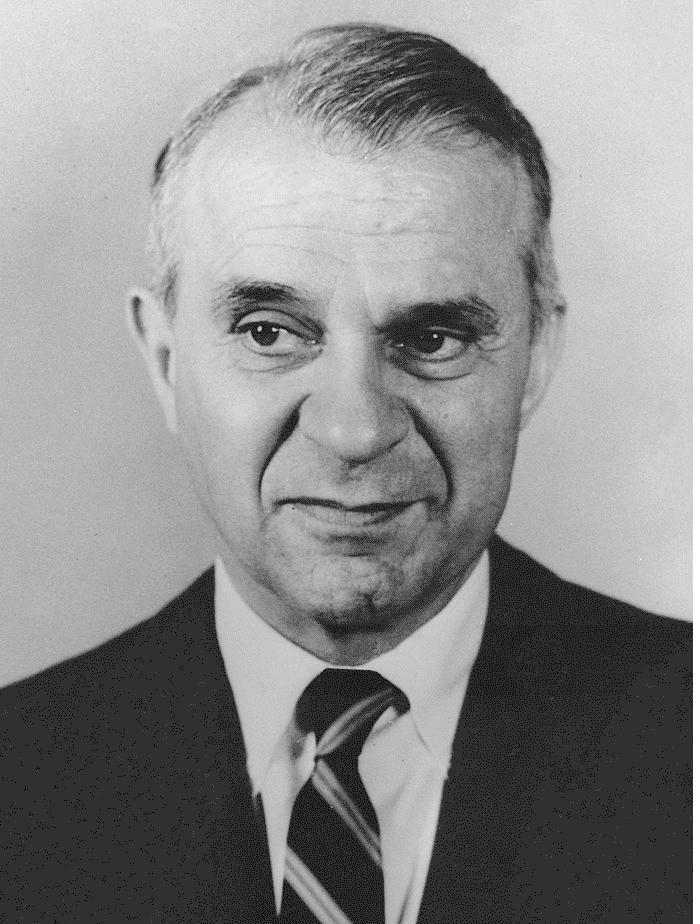
\includegraphics[width=6cm]{images/LEONTIEF}};
\end{tikzpicture}
\end{center}

\vspace{4mm}

\begin{center}
{\displayfont\fontsize{24}{28}\selectfont\color{SEGreen}Appendix B\par}
\vspace{2mm}
{\displayfont\fontsize{18}{22}\selectfont\color{SESubtitle}Data and Hypotheses\par}
\vspace{2mm}
{\fontsize{9}{11}\selectfont\color{SESubtitle}Wassily Leontief (1906--1999)\par}
\end{center}

\vspace{4mm}

\begin{pullquote}
The data for a particular year, set out in the form of a rectangular input-output table, describe the flows of goods and services among all sectors of an economy.
\end{pullquote}

\vspace{4mm}

\begin{twocolbody}
\noindent The empirical foundation of this study rests on a geocoded database of 8,572 installed data centers across 120 countries (90.8~GW), linked to facility-level financial parameters, CMIP climate projections, and three AI-era growth scenarios. This appendix documents model architecture, database construction, financial calibration, physical risk data, supply chain propagation (Leontief input-output), and output data---enabling full reproducibility.

\subsubsection*{Contents}
\begin{itemize}[leftmargin=10pt, itemsep=2pt]
  \item B.1 Model architecture and database construction
  \item B.2 Financial parameter calibration
  \item B.3 Physical risk data and supply chain data
  \item B.4 Output data and parameter confidence
\end{itemize}
\end{twocolbody}

% --- Full content from working paper appendix ---
\clearpage
% =============================================================================
% APPENDIX A: DATA AND HYPOTHESES
% Last updated: 2026-03-06
% =============================================================================

\section{Data and Hypotheses}

% =============================================
% A.1 MODEL ARCHITECTURE
% =============================================

\subsection{Model Architecture}
\label{app:model_arch}

The analysis is built from a structured input system containing 17 interconnected
components that form the complete hypothesis chain. The architecture is designed for
transparency and reproducibility: every numerical assumption is stored in a single
documented location, and modifying any parameter triggers automatic recalculation of
all downstream outputs.

\begin{table}[H]
\centering
\footnotesize
\caption{Model input architecture --- 17 components}
\label{tab:app_sheets}
\renewcommand{\arraystretch}{1.2}
\begin{tabular}{@{}p{3.8cm}p{2cm}p{7.5cm}@{}}
\toprule
\textbf{Component} & \textbf{Category} & \textbf{Content} \\
\midrule
Scenario definitions & Documentation & Model version history (V5--V7), scenario structure, changelog \\
Data flow architecture & Documentation & Dependency map across all input and output components \\
Global parameters & Hypotheses & 29 modifiable parameters: asset valuation, operating ratios, growth, depreciation \\
Carbon decoupling ratios & Hypotheses & Carbon/revenue trajectories by region $\times$ scenario (2025--2050) \\
Source traceability & Hypotheses & Literature references and confidence ratings for each parameter \\
Country financial data & Parameters & 120 countries: grid carbon intensity (5 horizons), tax, COGS, OPEX, WACC \\
Facility database & Core data & 13{,}205 geocoded facilities $\times$ 64 attributes \\
Efficiency matrices & Parameters & PPA factors and PUE by region $\times$ facility tier, with dynamic trajectories \\
Regional carbon projections & Trajectories & MW-weighted regional carbon intensity to 2050 \\
Aggregate results & Outputs & ClimVaR by scenario, region, channel, adaptation pathway \\
Efficiency sensitivity & Outputs & Sensitivity of results to PPA and PUE parameter variation \\
Regional decomposition & Outputs & Portfolio, ClimVaR$\times$region, facility type, channels, risk tiers \\
IEA reference mapping & Calibration & IEA source citations with section-level traceability \\
AI demand projections & Calibration & IEA electricity demand under three AI growth scenarios \\
Grid supply mix & Calibration & Regional generation mix projections to 2050 \\
Emissions cross-check & Calibration & Modeled emissions validated against IEA benchmarks \\
Extended risk parameters & Calibration & Grid delay, electricity price multipliers, supply chain data \\
\bottomrule
\end{tabular}
\end{table}

The model has undergone four documented version increments. Version~5 introduced dynamic
IEA trajectories replacing static parameters. Version~6 added regionalized asset values,
cooling ratios, and grid congestion modeling. Version~7 computed facility-level ClimVaR
across all scenarios, producing 24 output columns per facility (4 scenario combinations
$\times$ 6 channel metrics). Version~7.5 integrated three AI growth scenarios with binary
inclusion flags, enabling portfolio-level analysis under LTG, SAI, and AWB assumptions
from a single database.


% =============================================
% A.2 FACILITY DATABASE
% =============================================

\subsection{Facility Database}
\label{app:database}

\subsubsection{Database Dimensions}

The core facility database contains 13{,}205 rows and 64 columns. Each row represents
a single data center facility; each column carries one of six categories of information:

\begin{itemize}
\item \textbf{Location} (3 columns): geocoded latitude, longitude, and ISO country code
(120 countries represented).
\item \textbf{Identity and capacity} (8 columns): unique identifier, IT capacity (MW),
facility name, owner, provider type, sub-region, rack count, source database.
\item \textbf{Financial structure} (14 columns): annual revenue, asset value, COGS ratio,
OPEX ratio, tax rate, WACC, yearly growth, terminal growth, depreciation ratio, CAPEX
ratio, insurance premium, electricity cooling ratio, outdoor salary ratio, purchase ratio.
\item \textbf{Efficiency and emissions} (6 columns): Scope~1 emissions (tCO$_2$/yr),
Scope~2 raw and PPA-adjusted, PUE, PPA factor, and terminal value year.
\item \textbf{ClimVaR outputs} (24 columns): facility-level ClimVaR percentage and five
channel decompositions ($\gamma$, CC$^2$, $\beta$, $\delta$, $\xi$), under 4 scenario
combinations (BAU/NZT $\times$ MEAN/Q95).
\item \textbf{Scenario flags} (3 columns): binary inclusion flags for LTG, SAI, AWB
growth scenarios.
\end{itemize}


\subsubsection{Installed Base: Sources and Coverage}

The installed base comprises 8{,}572 facilities totaling 90{,}818~MW (90.8~GW),
assembled from four complementary source types:

\begin{enumerate}
\item \textbf{Commercial databases}: Data Center Map, Cloudscene, and proprietary
Schneider Electric client records provide the core inventory with location, operator,
and capacity attributes. Cross-referencing eliminates duplicates.
\item \textbf{Regulatory filings}: planning permissions, environmental impact assessments,
and grid connection applications in the US, EU, China, and Japan provide independent
capacity verification for facilities above 10~MW.
\item \textbf{Satellite imagery validation}: building footprint analysis provides
independent size estimates, calibrated against known facilities to derive MW capacity
from floor area.
\item \textbf{Operator disclosures}: annual and sustainability reports from publicly
listed operators (Equinix, Digital Realty, CyrusOne, NTT, Chindata, GDS) provide
facility-level data for approximately 35\% of total installed GW.
\end{enumerate}

\paragraph{Capacity distribution.} Facility IT capacities range from 15~kW (enterprise
server rooms) to 300~MW (hyperscale campuses), with a median of 10.6~MW. The distribution
is heavily right-skewed: 73.4\% of facilities exceed 1~MW, but only 4.7\% exceed 50~MW
and 3.0\% exceed 100~MW. The top decile by capacity accounts for over 60\% of total GW.

\begin{table}[H]
\centering
\small
\caption{Installed base capacity distribution}
\label{tab:app_mw_dist}
\begin{tabular}{@{}lrrr@{}}
\toprule
\textbf{Capacity band} & \textbf{Facilities} & \textbf{\% of base} & \textbf{Cumulative GW} \\
\midrule
$<$ 1 MW & 2{,}283 & 26.6\% & 0.9 \\
1--5 MW & 3{,}221 & 37.6\% & 9.5 \\
5--10 MW & 906 & 10.6\% & 6.6 \\
10--50 MW & 1{,}755 & 20.5\% & 36.5 \\
50--100 MW & 152 & 1.8\% & 10.7 \\
$>$ 100 MW & 255 & 3.0\% & 26.6 \\
\midrule
\textbf{Total} & \textbf{8{,}572} & \textbf{100\%} & \textbf{90.8} \\
\bottomrule
\end{tabular}
\end{table}

\paragraph{Provider types.} The database classifies facilities into five provider
categories reflecting operational characteristics and financial profiles.

\begin{table}[H]
\centering
\small
\caption{Installed base by provider type}
\label{tab:app_provider}
\begin{tabular}{@{}lrrl@{}}
\toprule
\textbf{Provider type} & \textbf{Facilities} & \textbf{\% of base} & \textbf{Typical capacity} \\
\midrule
Retail colocation & 5{,}662 & 66.1\% & 0.015--5~MW \\
Wholesale / large colocation & 1{,}560 & 18.2\% & 5--50~MW \\
Telecommunications & 1{,}068 & 12.5\% & 0.5--20~MW \\
Hyperscale (cloud) & 149 & 1.7\% & 50--300~MW \\
Other (hosting, reseller, cloud) & 133 & 1.6\% & Variable \\
\bottomrule
\end{tabular}
\end{table}

\paragraph{Country coverage.} Table~\ref{tab:app_country_coverage} presents the 20
largest data center markets by installed capacity. Together they account for 93\% of
global installed MW. The full database covers 120 countries.

\begin{table}[H]
\centering
\small
\caption{Top 20 data center markets by installed capacity}
\label{tab:app_country_coverage}
\begin{tabular}{@{}lrrr|lrrr@{}}
\toprule
\textbf{Country} & \textbf{DCs} & \textbf{MW} & \textbf{\%} & \textbf{Country} & \textbf{DCs} & \textbf{MW} & \textbf{\%} \\
\midrule
United States & 2{,}383 & 30{,}329 & 33.4 & Canada & 272 & 1{,}327 & 1.5 \\
China & 1{,}284 & 25{,}076 & 27.6 & Russia & 255 & 1{,}054 & 1.2 \\
United Kingdom & 374 & 3{,}596 & 4.0 & South Korea & 94 & 1{,}023 & 1.1 \\
Japan & 447 & 2{,}940 & 3.2 & Norway & 27 & 896 & 1.0 \\
India & 206 & 2{,}603 & 2.9 & Hong Kong & 109 & 809 & 0.9 \\
Germany & 291 & 2{,}128 & 2.3 & UAE & 49 & 775 & 0.9 \\
France & 186 & 1{,}682 & 1.9 & Israel & 61 & 739 & 0.8 \\
Australia & 247 & 1{,}624 & 1.8 & Italy & 151 & 716 & 0.8 \\
Singapore & 115 & 1{,}547 & 1.7 & Brazil & 116 & 683 & 0.8 \\
Ireland & 63 & 1{,}542 & 1.7 & Netherlands & 207 & 1{,}434 & 1.6 \\
\bottomrule
\end{tabular}
\end{table}

\paragraph{Aggregate emissions.} The installed base generates approximately 1.0~MtCO$_2$/yr
in Scope~1 emissions (diesel backup) and 482.7~MtCO$_2$/yr in raw Scope~2 emissions
(purchased electricity). After PPA adjustment, Scope~2 decreases to 400.0~MtCO$_2$/yr
(17\% reduction). Total annual revenue is \$147~billion; total book asset value is
\$750~billion.


\subsubsection{Prospective AI-Era Infrastructure}

Prospective facilities are drawn from four source databases, ordered by decreasing certainty.

\begin{table}[H]
\centering
\small
\caption{Prospective facility source databases}
\label{tab:app_source_databases}
\begin{tabular}{@{}p{4cm}rrrl@{}}
\toprule
\textbf{Source} & \textbf{Facilities} & \textbf{GW} & \textbf{Mean MW} & \textbf{Certainty} \\
\midrule
Epoch AI GPU Clusters & 62 & 7.8 & 125 & High \\
Tier~2 Announced & 46 & 4.6 & 100 & Medium \\
Probabilistic LTG & 2{,}316 & 231.3 & 100 & Low \\
Probabilistic SAI & 2{,}195 & 219.1 & 100 & Low \\
\bottomrule
\end{tabular}
\end{table}

\small\textit{The total unique database contains 4{,}633 prospective facilities (462.7~GW).
Facilities are assigned to growth scenarios via binary inclusion flags. The effective
count per scenario is: LTG = 615 (62.9~GW), SAI = 1{,}195 (121.1~GW), AWB = 2{,}939
(295.6~GW). Results in Parts~IV--VI are reported by scenario, not for the raw total.}
\normalsize

\paragraph{Tier~1 confirmed projects (sample).} The Epoch AI GPU Cluster database
includes named, publicly documented projects: OpenAI Stargate (Abilene TX, phased to
500~MW), Microsoft AI campuses (UK, Sweden, Spain), Meta superclusters (multiple US
locations), xAI Memphis (500~MW announced), NVIDIA Blackwell clusters (multiple sites),
AWS sovereign deployments (Saudi Arabia, Malaysia, Thailand, New Zealand, Chile), and
Google APAC expansion projects. These represent the highest-certainty prospective
capacity---most are under construction or recently commissioned.

\paragraph{Tier~2 announced projects (sample).} Includes sovereign AI campuses
(Sesterce Valence FR 250~MW, DataVolt NEOM SA 1.5~GW phased), large colocation expansions
with planning permissions (Pure DC UK, Vantage \$2B deployment, Brookfield \$10B plan),
and national programs (SK 3~GW plan South Korea, Scala 4.75~GW Brazil).


\subsubsection{Scenario Composition}

\begin{table}[H]
\centering
\small
\caption{Portfolio composition by AI growth scenario}
\label{tab:app_scenario_composition}
\begin{tabular}{@{}lrrrr@{}}
\toprule
\textbf{Scenario} & \textbf{Total DCs} & \textbf{Total GW} & \textbf{AI added} & \textbf{AI GW} \\
\midrule
Installed only & 8{,}572 & 90.8 & --- & --- \\
+ Limits to Growth & 9{,}187 & 153.7 & 615 & 62.9 \\
+ Sustainable AI & 9{,}767 & 211.9 & 1{,}195 & 121.1 \\
+ Abundance Without Boundaries & 11{,}511 & 386.4 & 2{,}939 & 295.6 \\
\bottomrule
\end{tabular}
\end{table}


\subsubsection{Regional Distribution}

\begin{table}[H]
\centering
\small
\caption{Facility coverage by region}
\label{tab:app_regional}
\begin{tabular}{@{}lrr|rr@{}}
\toprule
& \multicolumn{2}{c|}{\textbf{Installed base}} & \multicolumn{2}{c}{\textbf{Total (AWB)}} \\
\textbf{Region} & \textbf{DCs} & \textbf{GW} & \textbf{DCs} & \textbf{GW} \\
\midrule
United States & 2{,}383 & 30.3 & 4{,}071 & 199.1 \\
China & 1{,}284 & 25.1 & 2{,}267 & 123.4 \\
Europe & 2{,}019 & 15.4 & 2{,}574 & 70.9 \\
Asia-Pacific & 1{,}593 & 11.6 & 2{,}495 & 101.2 \\
Middle East & 255 & 2.6 & 370 & 14.1 \\
Rest of World & 1{,}038 & 5.9 & 1{,}428 & 44.9 \\
\midrule
\textbf{Total} & \textbf{8{,}572} & \textbf{90.8} & \textbf{11{,}511} & \textbf{386.4} \\
\bottomrule
\end{tabular}
\end{table}

\small\textit{Asia-Pacific excludes China; includes Japan, Australia, Singapore, South Korea.
Rest of World includes India, Canada, Latin America, Africa, Russia.}
\normalsize


\subsubsection{Geocoding and Climate Linkage}

All facilities are geocoded to coordinates enabling linkage to downscaled CMIP6 climate
projections at $0.1° \times 0.1°$ resolution ($\sim$10~km). For installed facilities,
coordinates are derived from address geocoding or satellite imagery. For prospective
facilities, coordinates are assigned at the announced site location (Tier~1/2) or
metropolitan area centroid (probabilistic). The climate linkage assigns four physical risk
variables to each facility for each year (2025--2050) under each RCP pathway at three
distribution quantiles (Q25, MEAN, Q95).


% =============================================
% A.3 FINANCIAL PARAMETERS
% =============================================

\subsection{Financial Parameter Calibration}
\label{app:financial}

\subsubsection{Global Parameters}

\begin{table}[H]
\centering
\footnotesize
\caption{Global model parameters (29 documented hypotheses)}
\label{tab:app_global_params}
\renewcommand{\arraystretch}{1.15}
\begin{tabular}{@{}p{4cm}rlll@{}}
\toprule
\textbf{Parameter} & \textbf{Value} & \textbf{Unit} & \textbf{Source} & \textbf{Confidence} \\
\midrule
Asset value / MW (base) & 9 & \$M/MW & Schneider, CBRE 2024 & High \\
PUE (global default) & 1.40 & --- & Uptime Institute 2024 & High \\
Backup ratio (diesel) & 0.50 & --- & Industry standard & High \\
Diesel consumption & 300 & L/MWh & Generator spec & High \\
Diesel emission factor & 2.68 & kgCO$_2$/L & GHG Protocol & High \\
AI revenue multiplier & 2.0$\times$ & --- & McKinsey, Thunder Said & Mixed \\
Size mult.\ (retail) & 1.0$\times$ & --- & Baseline & High \\
Size mult.\ (wholesale) & 0.87$\times$ & --- & CBRE, Houlihan Lokey & High \\
Size mult.\ (hyperscale) & 0.75$\times$ & --- & CBRE, Synergy Research & High \\
Revenue growth & 5\%/yr & --- & Industry consensus & Mixed \\
Terminal growth & 2\% & --- & Standard DCF & High \\
Elec.\ cooling / revenue & 5\% & --- & Uptime, IEA 2025 & Mixed \\
Outdoor salary / revenue & 0.4\% & --- & Expert estimate & Low \\
Purchase ratio ($p$) & 15\% & --- & $p \approx c - s$ & Mixed \\
Insurance premium (base) & 5\% & of damage & Industry standard & Mixed \\
Insurance premium (AI) & 10\% & of damage & Expert estimate & Low \\
Depreciation / AV ($d$) & 8\% & --- & Damodaran, Equinix & High \\
CAPEX / revenue (base) & 10\% & --- & CBRE mature DC & High \\
CAPEX / revenue (AI tiers) & 20\% & --- & Equinix 32\%, DLR 27\% & Mixed \\
\bottomrule
\end{tabular}
\end{table}


\subsubsection{Asset Valuation by Region and Tier}

\begin{table}[H]
\centering
\small
\caption{Asset value per MW (\$M/MW) by region and facility tier}
\label{tab:app_asset_value}
\begin{tabular}{@{}lccccl@{}}
\toprule
\textbf{Region} & \textbf{Base} & \textbf{Tier1} & \textbf{Tier2} & \textbf{Tier3} & \textbf{Rationale} \\
\midrule
US & 9 & 40 & 25 & 30 & Highest construction costs \\
Europe & 9 & 38 & 24 & 28 & $\sim$95\% of US costs \\
China & 7 & 28 & 18 & 22 & $\sim$70\% of US costs \\
Asia-Pacific & 8 & 32 & 20 & 25 & Mix SG/JP (high) + ID/TH (low) \\
Middle East & 9 & 42 & 26 & 32 & Extreme heat cooling premium \\
RoW & 8 & 30 & 20 & 24 & Mixed; LatAm $\sim$85\% of US \\
\bottomrule
\end{tabular}
\end{table}

\small\textit{Sources: IEA (2025); Schneider Electric TradeOff Tool; CBRE 2024. Tier1 upper
bound (\$42M/MW, Middle East) reflects IEA frontier AI estimates.}
\normalsize

\vspace{0.2cm}
The base asset value of \$9M/MW produces a total installed book value of \$750~billion.
Size multipliers and the AI revenue multiplier produce an effective range from \$6.8M/MW
(large legacy wholesale) to \$42M/MW (Tier~1 AI, Middle East). The DCF valuation ($V_0$)
exceeds book value by approximately $\times$1.35 for the installed base (\$1{,}012B on
\$750B), reflecting the going-concern premium of operational facilities.


\subsubsection{Observed Parameter Ranges}

Table~\ref{tab:app_ranges} reports the actual ranges computed across all 13{,}205
facilities, validating that calibration produces realistic distributions.

\begin{table}[H]
\centering
\small
\caption{Observed parameter ranges across the database}
\label{tab:app_ranges}
\begin{tabular}{@{}lrrrr@{}}
\toprule
\textbf{Parameter} & \textbf{Min} & \textbf{Median} & \textbf{Max} & \textbf{Unit} \\
\midrule
IT capacity & 0.015 & 11.2 & 300.0 & MW \\
Asset value & \$120K & \$91M & \$8.0B & \$ \\
Annual revenue & \$29K & \$18.8M & \$720M & \$/yr \\
COGS / revenue & 35\% & 46\% & 50\% & ratio \\
OPEX / revenue & 22\% & 27\% & 30\% & ratio \\
WACC & 5.5\% & 7.0\% & 15.5\% & ratio \\
Tax rate & 0\% & 25\% & 35\% & ratio \\
PUE & 1.12 & 1.40 & 1.55 & ratio \\
PPA factor & 0.49 & 0.70 & 0.90 & ratio \\
ClimVaR\% (BAU/MEAN) & 2.4\% & 8.8\% & 16.3\% & \% of $V_0$ \\
ClimVaR\% (NZT/MEAN) & 3.0\% & 9.7\% & 17.0\% & \% of $V_0$ \\
\bottomrule
\end{tabular}
\end{table}


\subsubsection{Country-Level Parameters}

The model provides 14 parameters for each of 120 countries: grid carbon intensity at five
time horizons (2024, 2030, 2035, 2040, 2050), tax rate, COGS ratio, OPEX ratio, WACC, and
regional classification. Table~\ref{tab:app_country_full} presents the 20 largest markets.

\begin{table}[H]
\centering
\footnotesize
\caption{Financial and carbon parameters --- 20 largest data center markets}
\label{tab:app_country_full}
\begin{tabular}{@{}l r rrrrr rrr@{}}
\toprule
& & \multicolumn{5}{c}{\textbf{Grid carbon intensity (gCO$_2$/kWh)}} & & & \\
\cmidrule(lr){3-7}
\textbf{Country} & \textbf{Region} & \textbf{2024} & \textbf{2030} & \textbf{2035} & \textbf{2040} & \textbf{2050} & \textbf{Tax} & \textbf{COGS} & \textbf{WACC} \\
\midrule
US & N.\ Am. & 390 & 293 & 215 & 156 & 120 & 21\% & 48\% & 6.8\% \\
CN & AP Em. & 580 & 464 & 348 & 232 & 136 & 25\% & 38\% & 9.0\% \\
DE & W.\ Eur. & 380 & 247 & 160 & 106 & 46 & 30\% & 49\% & 6.5\% \\
GB & W.\ Eur. & 220 & 143 & 93 & 62 & 26 & 25\% & 47\% & 7.2\% \\
JP & AP Dev. & 470 & 329 & 235 & 188 & 141 & 30\% & 48\% & 6.5\% \\
FR & W.\ Eur. & 55 & 36 & 23 & 15 & 7 & 25\% & 44\% & 6.8\% \\
SG & AP Dev. & 420 & 294 & 210 & 168 & 126 & 17\% & 45\% & 6.0\% \\
IN & S.\ Asia & 710 & 533 & 391 & 284 & 178 & 25\% & 35\% & 11.5\% \\
AU & AP Dev. & 620 & 496 & 372 & 260 & 136 & 30\% & 44\% & 7.2\% \\
NL & W.\ Eur. & 310 & 202 & 131 & 87 & 37 & 26\% & 47\% & 6.5\% \\
BR & Lat.\ Am. & 90 & 74 & 57 & 45 & 25 & 34\% & 40\% & 11.5\% \\
KR & AP Dev. & 450 & 315 & 225 & 180 & 90 & 24\% & 44\% & 6.5\% \\
IE & W.\ Eur. & 300 & 195 & 126 & 84 & 36 & 12\% & 47\% & 7.0\% \\
AE & M.\ East & 400 & 352 & 288 & 232 & 140 & 9\% & 36\% & 8.0\% \\
SE & W.\ Eur. & 15 & 10 & 6 & 4 & 3 & 21\% & 47\% & 6.5\% \\
NO & W.\ Eur. & 10 & 7 & 4 & 3 & 2 & 22\% & 47\% & 6.5\% \\
MY & AP Em. & 550 & 413 & 303 & 220 & 110 & 24\% & 38\% & 8.5\% \\
ID & AP Em. & 700 & 560 & 420 & 280 & 168 & 22\% & 35\% & 10.0\% \\
SA & M.\ East & 500 & 440 & 360 & 290 & 175 & 20\% & 40\% & 8.5\% \\
MX & Lat.\ Am. & 440 & 330 & 242 & 176 & 110 & 30\% & 42\% & 10.0\% \\
\bottomrule
\end{tabular}
\end{table}

\small\textit{Grid carbon intensity: IEA (2025) regional projections. Tax: OECD (2024).
COGS: Equinix, Digital Realty, CyrusOne reports. WACC: Damodaran (2024) REIT sector
with country risk premiums. The 100 remaining countries follow the same structure.}
\normalsize


% =============================================
% A.4 PHYSICAL RISK DATA
% =============================================

\newpage
\subsection{Physical Risk Data}
\label{app:physical}

\subsubsection{Climate Projection Source}

Physical risk variables are extracted from bias-corrected, statistically downscaled CMIP6
projections \citep{eyring2016} at $0.1° \times 0.1°$ resolution ($\sim$10~km at
mid-latitudes). Projections are generated at each facility's geocoded coordinates for
2025--2050 under RCP~2.6, 4.5, and 8.5, at three distribution quantiles (Q25, MEAN, Q95).

\subsubsection{Variable Definitions}

\begin{table}[H]
\centering
\small
\caption{Physical risk variables: definitions and channel mapping}
\label{tab:app_physical_vars}
\begin{tabular}{@{}p{2.2cm}p{1.5cm}p{4cm}p{5.5cm}@{}}
\toprule
\textbf{Variable} & \textbf{Channel} & \textbf{Definition} & \textbf{Climate driver} \\
\midrule
COOLING & $\gamma$ & Fractional increase in cooling energy vs.\ 2024 & Cooling degree days (CDD, base 18°C, ASHRAE) \\
BID & $\beta$ & Business interruption days/yr, fraction of year & Composite: flood, storm, drought, wildfire, heat \\
DAMAGE & $\delta$ & Annual damage probability, fraction of AV & Flood depth, wind speed, seismic, fire \\
HPL & $\xi$ & Fractional outdoor labor productivity loss & Days $>$ 35°C / 40°C wet-bulb \\
\bottomrule
\end{tabular}
\end{table}

\subsubsection{Hazard Sub-Decomposition}

For the business interruption and damage channels, the model further decomposes risk into
five hazard types: drought (d), extreme wind (ew), riverine flood (r), storm surge (s),
and tropical wind (tw). This decomposition provides the inputs for the Shapley attribution
(Section~2.2.3) and is reported at facility level in the case study outputs. Each hazard
type carries its own annual probability distribution at facility coordinates.

\subsubsection{Dataset Scale}

The complete projection dataset contains approximately 17~million observations:
up to 11{,}511 facilities (AWB) $\times$ 25 years $\times$ 2--3 RCP pathways $\times$
4 physical risk variables $\times$ 3 quantiles. Projections are computed for all facilities
regardless of scenario inclusion, enabling flexible portfolio composition at analysis stage.


% =============================================
% A.5 SUPPLY CHAIN DATA
% =============================================

\subsection{Supply Chain Data}
\label{app:supply_chain}

\subsubsection{Leontief Input-Output Tables}

The technical coefficient matrix $A$ is drawn from OECD Multi-Regional Input-Output Tables
(MRIOT, 2019 vintage): 67 countries $\times$ 45 ISIC sectors. The data center sector maps
to ISIC telecommunications, computer services, and electrical equipment manufacturing.

\subsubsection{Supply Chain Concentration}

\begin{table}[H]
\centering
\small
\caption{Critical supply chain components for data center infrastructure}
\label{tab:app_supply_chain}
\begin{tabular}{@{}p{3cm}cp{2.5cm}p{2cm}p{3.5cm}@{}}
\toprule
\textbf{Component} & \textbf{China share} & \textbf{Category} & \textbf{Substitut.} & \textbf{DC impact} \\
\midrule
GaN devices & 99\% & Semiconductors & Very low & Power conversion \\
High-purity Si (4N+) & 95\% & Raw material & Very low & Semiconductor base \\
Rare earth magnets & 90\% & Cooling & Very low & Fans, pumps, compressors \\
LFP battery cells & 99\% & Storage & Low & UPS, BESS \\
SiC substrates & 50\% & Semiconductors & Medium & Power supply \\
HBM memory & $\sim$40\% (KR) & Memory & Low & GPU bandwidth \\
Refined copper & 40\% & Cabling/cooling & Medium & Busbars, heat exchangers \\
Transformers & $\sim$35\% & Grid equipment & Medium & DC power feed \\
\bottomrule
\end{tabular}
\end{table}

\small\textit{Sources: IEA (2025) Table 4.1; IEA Critical Minerals; USGS.}
\normalsize

\subsubsection{Pass-Through Calibration}

\begin{table}[H]
\centering
\small
\caption{Leontief pass-through rates by supply chain pathway}
\label{tab:app_passthrough}
\begin{tabular}{@{}p{3.5cm}ccp{5cm}@{}}
\toprule
\textbf{Pathway} & \textbf{Rate} & \textbf{Lead time} & \textbf{Rationale} \\
\midrule
Semiconductor fab & 60--80\% & 6--12 mo & TSMC 54\%, limited substitutability \\
Power transformers & 40--60\% & 18--36 mo & Moderate concentration, long lead \\
Cooling components & 20--40\% & 3--6 mo & More substitutable \\
Server/rack assembly & 30--50\% & 3--9 mo & Component bottlenecks \\
\bottomrule
\end{tabular}
\end{table}

\small\textit{Calibrated from: \citet{barrot2016}, IEA \citep{iea2025energyai}, expert assessment.
Fixed-coefficient limitation discussed in Section~5.10.}
\normalsize


% =============================================
% A.6 OUTPUT DATA STRUCTURE
% =============================================

\subsection{Output Data Structure}
\label{app:outputs}

The model produces three output datasets, documented in Table~\ref{tab:app_outputs}.

\begin{table}[H]
\centering
\footnotesize
\caption{Model output datasets}
\label{tab:app_outputs}
\renewcommand{\arraystretch}{1.2}
\begin{tabular}{@{}p{2.8cm}p{1.3cm}p{1.3cm}p{8cm}@{}}
\toprule
\textbf{Dataset} & \textbf{Rows} & \textbf{Cols} & \textbf{Content} \\
\midrule
Aggregate results & 288 & 14 & ClimVaR by scenario (BAU/NZT) $\times$ quantile (Q25/MEAN/Q95) $\times$ region (4) $\times$ asset class (4) $\times$ adaptation (3). Columns: $V_0$, five channels, residual value, ClimVaR\%, ClimVaR. \\[0.2cm]
Annual decomposition & 288 & 305 & Same cross-section with annual resolution 2026--2050. 12 channel variables $\times$ 25 years + 3 annual summary metrics $\times$ 25 years. Enables trajectory analysis. \\[0.2cm]
Facility case studies & 72 & 592 & Three sites (Abilene, Valence, Guangdong) $\times$ 24 scenario combinations. 64 base columns + 528 time-series columns: 22 channel-hazard decompositions $\times$ 25 years. \\
\bottomrule
\end{tabular}
\end{table}

The 12 channel variables decompose ClimVaR into: direct business interruption, supply
chain interruption, physical damage (by 5 hazard types: drought, extreme wind, riverine
flood, storm surge, tropical wind), heat productivity, cooling cost increase, and carbon
costs (Scopes 1, 2, 3). The facility case study dataset further decomposes damage into the
same five hazard types, enabling the Shapley attribution presented in Section~4.3.


% =============================================
% A.7 PARAMETER CONFIDENCE
% =============================================

\subsection{Parameter Confidence and Sensitivity}
\label{app:confidence}

Of the 29 documented global parameters, 14 (48\%) are calibrated directly from published
data with high confidence, 10 (34\%) combine literature and expert judgment, and 5 (17\%)
rely primarily on expert estimates. The low-confidence parameters are minor contributors:
a $\pm$50\% perturbation of all five changes aggregate ClimVaR by $<$3\%.

\subsubsection{Validation Cross-Checks}

\paragraph{Industry benchmark.} The WEF projects climate-driven costs for data centers of
\$81~billion annually by 2035 \citep{wef2025}. Our installed base ClimVaR of \$388~billion,
annualized over 25 years at 7\% discount rate, implies approximately \$34~billion/yr---lower
than the WEF figure (which includes prospective infrastructure). Under Abundance Without
Boundaries, our annualized equivalent rises to $\sim$\$150~billion. Directional alignment
confirms that ClimVaR values are conservative.

\paragraph{Sensitivity bounds.} WACC $\pm$2~pp shifts aggregate ClimVaR by $\pm$15--20\%;
halving BI frequency reduces it by $\sim$25\%; $\pm$50\% on the five low-confidence
parameters changes aggregate ClimVaR by $<$3\%. The order of magnitude ($\sim$\$400B
installed) is robust to reasonable parameter variation. Monte Carlo sensitivity analysis
is planned for a subsequent version.

% =============================================================================
% APPENDIX C — Markowitz (Adaptation / Scenarios)
% =============================================================================
\clearpage\thispagestyle{chapterstart}

\begin{center}
\begin{tikzpicture}
  \clip (0,0) circle (3cm);
  \node[inner sep=0pt] at (0,0) {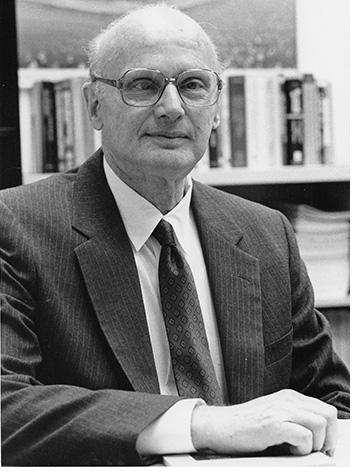
\includegraphics[width=6cm]{images/MARKOWITZ}};
\end{tikzpicture}
\end{center}

\vspace{4mm}

\begin{center}
{\displayfont\fontsize{24}{28}\selectfont\color{SEGreen}Appendix C\par}
\vspace{2mm}
{\displayfont\fontsize{18}{22}\selectfont\color{SESubtitle}Scenario Architecture\par}
\vspace{2mm}
{\fontsize{9}{11}\selectfont\color{SESubtitle}Harry Markowitz (1927--2023)\par}
\end{center}

\vspace{4mm}

\begin{pullquote}
Diversification is both observed and sensible; a rule of behavior which does not imply the superiority of diversification must be rejected both as a hypothesis and as a maxim.
\end{pullquote}

\vspace{4mm}

\begin{twocolbody}
\noindent Adaptation investment across a portfolio of data centers mirrors the logic of financial portfolio theory. Operators allocate finite capital across facilities with heterogeneous risk profiles, seeking the combination that maximizes risk reduction per dollar invested.

The framework models three strategies---Baseline, Selective, and Proactive---and demonstrates that risk reductions are multiplicative, not additive, because channels interact through the Shapley decomposition. The ``one champion action'' approach (Selective) targets the highest-Shapley-value channel per facility.

\subsubsection*{Contents}
\begin{itemize}[leftmargin=10pt, itemsep=2pt]
  \item C.1 Climate-economic pathways (BAU, NZT)
  \item C.2 AI growth scenarios (LTG, SAI, AWB)
  \item C.3 Risk channel trajectories (2026--2050)
  \item C.4 Adaptation parameters and non-additivity
\end{itemize}
\end{twocolbody}

% --- Full scenario content from working paper ---
\clearpage
% =============================================================================
% APPENDIX C: SCENARIO ARCHITECTURE AND RISK MODELING
% Trajectories, adaptation parameters, physical and transition risk modeling
% Last updated: 2026-03-06
% =============================================================================
\newpage
\section{Scenario Architecture}
\label{app:scenarios}

% =============================================
% C.1 EFFICIENCY AND EMISSIONS TRAJECTORIES
% =============================================

\subsection{Efficiency and Emissions Trajectories}
\label{app:efficiency}

\subsubsection{PPA Factor Trajectories}

PPA factors represent the fraction of grid emissions retained after renewable procurement
(1.0 = fully grid-dependent; 0.0 = fully renewable). They decline over time as renewable
procurement expands, at different rates by region reflecting market maturity and policy
environment.

\begin{table}[H]
\centering
\small
\caption{PPA factor trajectories by region (base facilities, BAU pathway, 2024--2050)}
\label{tab:app_ppa_traj}
\begin{tabular}{@{}lcccccl@{}}
\toprule
\textbf{Region} & \textbf{2024} & \textbf{2030} & \textbf{2035} & \textbf{2040} & \textbf{2045} & \textbf{2050} \\
\midrule
US & 0.70 & 0.55 & 0.42 & 0.32 & 0.25 & 0.20 \\
Europe & 0.65 & 0.48 & 0.33 & 0.22 & 0.16 & 0.12 \\
China & 0.85 & 0.78 & 0.65 & 0.52 & 0.44 & 0.38 \\
Asia-Pacific & 0.80 & 0.68 & 0.55 & 0.42 & 0.35 & 0.30 \\
Middle East & 0.90 & 0.80 & 0.65 & 0.50 & 0.42 & 0.35 \\
RoW & 0.90 & 0.85 & 0.75 & 0.62 & 0.54 & 0.48 \\
\bottomrule
\end{tabular}
\end{table}

\small\textit{Tier multipliers: base $\times$1.0, tier1 $\times$0.75, tier2 $\times$0.80, tier3 $\times$0.85. Under NZT, decline is approximately 30\% steeper. Sources: IEA, RE100, BNEF 2024. Validated against IEA (2025) \S6: $\sim$40\% industry PPA coverage by 2027.}
\normalsize

\subsubsection{PUE Trajectories}

\begin{table}[H]
\centering
\small
\caption{PUE trajectories by region (base / tier1)}
\label{tab:app_pue}
\begin{tabular}{@{}lcc|cc|cc@{}}
\toprule
& \multicolumn{2}{c|}{\textbf{2024}} & \multicolumn{2}{c|}{\textbf{2035}} & \multicolumn{2}{c}{\textbf{2050}} \\
\textbf{Region} & \textbf{Base} & \textbf{Tier1} & \textbf{Base} & \textbf{Tier1} & \textbf{Base} & \textbf{Tier1} \\
\midrule
US & 1.45 & 1.15 & 1.24 & 1.10 & 1.12 & 1.06 \\
Europe & 1.40 & 1.12 & 1.20 & 1.08 & 1.10 & 1.05 \\
China & 1.50 & 1.18 & 1.28 & 1.11 & 1.14 & 1.06 \\
Asia-Pacific & 1.45 & 1.15 & 1.26 & 1.10 & 1.14 & 1.06 \\
Middle East & 1.55 & 1.20 & 1.32 & 1.12 & 1.16 & 1.07 \\
RoW & 1.55 & 1.20 & 1.32 & 1.12 & 1.16 & 1.07 \\
\bottomrule
\end{tabular}
\end{table}

\small\textit{Sources: Uptime Institute 2024 (industry avg = 1.56); Google sustainability reports (1.09); IEA (2025). China government mandates PUE $<$1.3 for new builds.}
\normalsize

\subsubsection{Carbon Ratio Trajectories}

The carbon ratio decouples carbon cost growth from revenue growth, capturing the combined effect of grid decarbonization, renewable procurement, and efficiency improvement:

$$\text{carbon\_ratio}(r, t) \approx \frac{I_{\text{carb}}(r, t)}{I_{\text{carb}}(r, 2024)} \times \frac{\text{PPA}(r, t)}{\text{PPA}(r, 2024)} \times \frac{\text{PUE}(r, t)}{\text{PUE}(r, 2024)}$$

\begin{table}[H]
\centering
\small
\caption{Carbon ratio trajectories (BAU / NZT)}
\label{tab:app_carbon_ratio}
\begin{tabular}{@{}lcc|cc|cc@{}}
\toprule
& \multicolumn{2}{c|}{\textbf{2030}} & \multicolumn{2}{c|}{\textbf{2040}} & \multicolumn{2}{c}{\textbf{2050}} \\
\textbf{Region} & \textbf{BAU} & \textbf{NZT} & \textbf{BAU} & \textbf{NZT} & \textbf{BAU} & \textbf{NZT} \\
\midrule
US & 0.92 & 0.82 & 0.75 & 0.48 & 0.62 & 0.25 \\
Europe & 0.85 & 0.75 & 0.58 & 0.35 & 0.42 & 0.15 \\
China & 0.95 & 0.88 & 0.78 & 0.55 & 0.62 & 0.32 \\
Asia-Pacific & 0.93 & 0.85 & 0.74 & 0.50 & 0.58 & 0.28 \\
Middle East & 0.96 & 0.88 & 0.76 & 0.52 & 0.56 & 0.28 \\
RoW & 0.97 & 0.92 & 0.84 & 0.65 & 0.68 & 0.40 \\
\bottomrule
\end{tabular}
\end{table}


% =============================================
% C.2 CARBON PRICE TRAJECTORIES
% =============================================

\subsection{Carbon Price Trajectories}
\label{app:carbon_price}

Carbon cost trajectories follow IEA scenarios \citep{iea2024}, differentiated by region and policy ambition.

\begin{table}[H]
\centering
\small
\caption{Carbon price trajectories by scenario and region (\$/tCO$_2$)}
\label{tab:app_carbon_price}
\begin{tabular}{@{}llccccc@{}}
\toprule
\textbf{Scenario} & \textbf{Region} & \textbf{2025} & \textbf{2030} & \textbf{2035} & \textbf{2040} & \textbf{2050} \\
\midrule
BAU & Europe (ETS) & 65 & 85 & 100 & 110 & 120 \\
 & China (ETS) & 10 & 25 & 40 & 55 & 80 \\
 & US (shadow) & 15 & 25 & 35 & 50 & 75 \\
 & RoW (effective) & 5 & 12 & 20 & 30 & 50 \\
\midrule
NZT & Europe (ETS) & 65 & 130 & 200 & 260 & 300 \\
 & China (ETS) & 10 & 50 & 100 & 160 & 250 \\
 & US (carbon tax) & 15 & 60 & 110 & 170 & 250 \\
 & RoW (effective) & 5 & 30 & 65 & 110 & 200 \\
\bottomrule
\end{tabular}
\end{table}

\small\textit{BAU reflects current policy trends. NZT follows NGFS Net Zero 2050. Under NZT, carbon costs multiply $\times$3--6 relative to BAU by 2050. Sources: NGFS Phase IV (2023), EU ETS market data, IEA WEO (2025).}
\normalsize

Carbon costs are allocated to three scopes following GHG Protocol definitions: Scope~1 covers direct emissions from diesel backup generators; Scope~2 covers purchased electricity, adjusted for grid carbon intensity by country and PPA factor; Scope~3 covers upstream supply chain emissions using Leontief propagation coefficients.


% =============================================
% C.3 ADAPTATION PARAMETERS
% =============================================

\subsection{Adaptation Parameters}
\label{app:adaptation}

\subsubsection{Reduction Rates by Channel}

\begin{table}[H]
\centering
\small
\caption{Adaptation reduction rates by channel and pathway}
\label{tab:app_adaptation}
\begin{tabular}{@{}lccl@{}}
\toprule
\textbf{Channel} & \textbf{Selective} & \textbf{Proactive} & \textbf{Primary mechanism} \\
\midrule
$\gamma$ Cooling & 15--25\% & 24\% & Liquid cooling adoption (immersion, DTC, CDU) \\
CC Carbon & 40--50\% & 63\% & Renewable PPAs + grid selection + on-site generation \\
$\beta$ Business Interruption & 10--20\% & 36\% & Microgrid + BESS + predictive monitoring \\
$\delta$ Physical Damage & 10--15\% & 24\% & Structural hardening + climate-aware siting \\
$\xi$ Heat Productivity & 10--15\% & 28\% & Automation + enclosed logistics + remote operations \\
\midrule
\textbf{Portfolio weighted} & \textbf{$\sim$21\%} & \textbf{$\sim$38\%} & \\
\bottomrule
\end{tabular}
\end{table}

\small\textit{Selective applies to new builds only (greenfield, +15--20\% CAPEX). Proactive applies across the portfolio including legacy retrofit (+40--60\% CAPEX). Reductions applied independently per channel. Interaction effects are partially captured but may be understated (see Section~5.10).}
\normalsize

\subsubsection{Adaptation Strategy Definitions}

Three pathways span the range from inaction to systematic portfolio integration:

\begin{itemize}
\item \textbf{Baseline}: No climate-specific adaptation. Air-cooled, grid-dependent, cost-optimized siting, no legacy retrofit. Represents the current industry default against which adaptation value is measured.

\item \textbf{Selective}: Climate-aware design for new builds only. Includes liquid cooling, climate-informed siting, and renewable PPAs for prospective facilities; legacy assets remain unchanged. Captures the ``low-regret'' adaptation available at greenfield stage. The Selective pathway captures approximately 56\% of total Proactive value at lower capital outlay.

\item \textbf{Proactive}: Systematic adaptation across the portfolio. Includes all Selective measures plus microgrid retrofit on legacy assets, geographic rebalancing of new capacity, structured adaptation programs incorporating energy services and monitoring, and consideration of early retirement for highest-risk facilities. Combines infrastructure technology solutions, energy strategy decisions, and portfolio management choices.
\end{itemize}


% =============================================
% C.4 PHYSICAL AND TRANSITION RISK MODELING
% =============================================

\subsection{Risk Channel Modeling}
\label{app:risk_modeling}

The mathematical derivation of how physical and transition risks enter the ClimVaR framework through the five channels ($\gamma$, CC$^{1,2,3}$, $\beta$, $\delta$, $\xi$) is provided in Appendix~B (Sections~B.6--B.9), including the Shapley decomposition for hazard attribution within the $\beta$ channel and the Leontief propagation for supply chain effects.

The key calibration result for transition risk: the combined PUE$\times$PPA adjustment reduces aggregate Scope~2 emissions from 2{,}888~MtCO$_2$/year (raw) to 1{,}841~MtCO$_2$/year (adjusted)---a 36\% reduction. Prospective AI facilities achieve approximately 50\% reduction; the installed base achieves approximately 17\%.

Physical and transition scenarios interact multiplicatively: RCP pathways set the hazard environment for physical channels; BAU/NZT pathways set carbon prices for transition channels; adaptation pathways modify both. The framework evaluates all combinations to identify robust strategies.

% =============================================================================
% APPENDIX D — Brundtland (Literature Review)
% =============================================================================
\clearpage\thispagestyle{chapterstart}

\begin{center}
\begin{tikzpicture}
  \clip (0,0) circle (3cm);
  \node[inner sep=0pt] at (0,0) {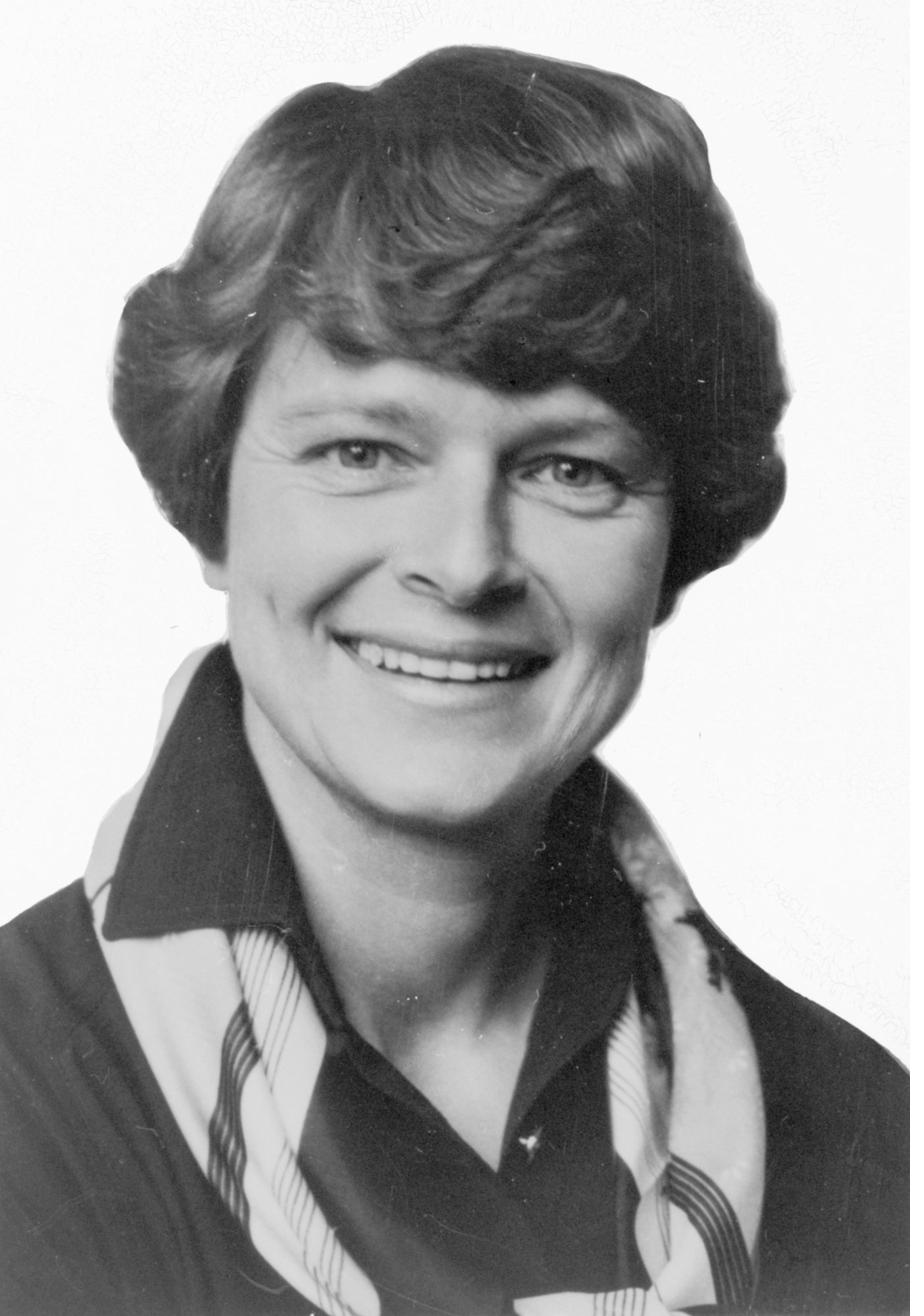
\includegraphics[width=6cm]{images/Brundtland}};
\end{tikzpicture}
\end{center}

\vspace{4mm}

\begin{center}
{\displayfont\fontsize{24}{28}\selectfont\color{SEGreen}Appendix D\par}
\vspace{2mm}
{\displayfont\fontsize{18}{22}\selectfont\color{SESubtitle}Literature Review\par}
\vspace{2mm}
{\fontsize{9}{11}\selectfont\color{SESubtitle}Gro Harlem Brundtland (b.\ 1939)\par}
\end{center}

\vspace{4mm}

\begin{pullquote}
Sustainable development is development that meets the needs of the present without compromising the ability of future generations to meet their own needs.
\end{pullquote}

\vspace{4mm}

\begin{twocolbody}
\noindent The empirical foundation rests on a geocoded database of 8,572 installed data centers across 120 countries (90.8~GW), linked to facility-level financial parameters, climate projections, and three AI-era growth scenarios. This appendix documents the literature context and reviews existing approaches to climate risk assessment for data centers and digital infrastructure.

\subsubsection*{Contents}
\begin{itemize}[leftmargin=10pt, itemsep=2pt]
  \item D.1 Physical climate risks for data centers
  \item D.2 Financial valuation of climate risk
  \item D.3 Infrastructure-specific assessment frameworks
  \item D.4 Gap analysis and positioning
\end{itemize}
\end{twocolbody}

% --- Full literature review from working paper ---
\clearpage
% =============================================================================
% APPENDIX D: LITERATURE REVIEW – CLIMATE RISK FOR DATA CENTERS
% Last updated: 2026-03-10
% =============================================================================

\section{Literature Review}
\label{app:literature}

Results are organised along three guiding questions:
(Q1) physical climate risks for data centers and digital infrastructure;
(Q2) insurance, insurability and climate risk for critical infrastructure;
(Q3) quantitative frameworks to integrate climate risk into infrastructure
valuation.

\subsection{Search Strategy and Screening Criteria}

The search process combined a broad semantic query on climate risk for data
centers and AI-related digital infrastructure with structured screening based
on abstracts and, where available, full texts. Papers and reports were
screened in when they met the following criteria:

\begin{itemize}
  \item \textbf{Infrastructure focus:} data centers, digital infrastructure,
        AI infrastructure, or closely related critical infrastructure
        (energy systems, telecommunications, industrial facilities, utilities).
  \item \textbf{Climate risk analysis:} quantitative modelling or analysis of
        physical climate risks (heat, flooding, storms, sea level rise, drought)
        and/or their economic or operational impacts.
  \item \textbf{Publication quality:} peer-reviewed academic papers or
        high-quality institutional reports from central banks, regulators,
        international organisations, or major research institutes.
  \item \textbf{Financial risk assessment:} explicit analysis of
        climate-related insurance, risk transfer, or methods for integrating
        climate risk into investment and financial assessment.
  \item \textbf{Infrastructure scale:} large-scale critical infrastructure
        rather than purely residential or small commercial buildings.
\end{itemize}

For each included study, we extracted information on infrastructure scope,
hazards, risk modelling approach, financial impacts, insurance treatment,
valuation framework, main findings, and acknowledged limitations.

\vspace{0.3cm}
\noindent The remainder of this appendix summarises the evidence base by
guiding question.

% =============================================
% D.1 Q1 – PHYSICAL CLIMATE RISKS
% =============================================

\subsection{Q1 – Physical Climate Risks for Data Centers and Digital Infrastructure}
\label{app:literature_q1}

The peer-reviewed literature directly quantifying physical climate risks for
data centers is extremely limited: only three studies explicitly address data
center siting and operations under climate change. A broader body of work on
analogous infrastructure — power generation, telecommunications, and
electricity grids — provides transferable methodologies. Flooding (riverine,
pluvial and coastal) emerges as the most consistently analysed hazard, with
heat extremes and storms also prominent. Most studies rely on RCP~4.5 and
RCP~8.5 (or SSP-equivalent) scenarios, with horizons extending from the 2030s
to 2100. Limitations repeatedly noted include coarse hazard-map resolution,
generic vulnerability functions not calibrated to local conditions, and
inadequate treatment of indirect impacts, cascading effects, and compound
hazards.

\subsubsection{Direct Data Center Studies}

\begin{table}[H]
\centering
\small
\caption{Direct data center climate risk studies}
\label{tab:app_lit_dc}
\begin{tabular}{@{}p{3.5cm}p{3.2cm}p{7.0cm}@{}}
\toprule
\textbf{Study} & \textbf{Scope} & \textbf{Key contributions and limitations} \\
\midrule
Pasupuleti (2022) &
Data center siting and capacity decisions &
Integrates HEC\textendash HMS hydrologic simulations into data center
location and capacity planning. Uses rainfall–runoff scenarios to estimate
flood probabilities and downtime risk, combined with CloudSim models to
quantify impacts on service availability and financial loss. Demonstrates a
rare linkage from hydrological hazards to operational disruptions; does not
yet include multi-hazard or insurance effects. \\[0.1cm]
Pasupuleti (2024) &
GIS-based siting under flood and climate risk &
Develops a climate- and flood-aware GIS framework for data center site
selection, incorporating riverine and pluvial flooding, sea-level rise, and
extreme precipitation. High-resolution DEMs and multi-criteria decision
analysis produce spatially explicit risk surfaces. Reports a 63\% reduction in
expected annual damage for hazard-aware siting relative to purely economic
criteria; vulnerability remains represented by generic damage functions. \\[0.1cm]
Pasupuleti (2025) &
GIS–AI framework for resilient siting and operation &
Combines climate datasets and machine learning models to build
risk-informed suitability surfaces and predict outage probability and cooling
energy demand. Shows that modest cost premiums for resilient locations can
be offset by reduced disruption and lower energy expenditure over asset
lifetimes. Focuses on siting and operation but does not quantify portfolio-level
financial tail risks. \\
\bottomrule
\end{tabular}
\end{table}

\subsubsection{Analogous Infrastructure with Transferable Methods}

\begin{table}[H]
\centering
\small
\caption{Representative climate risk studies for analogous infrastructure}
\label{tab:app_lit_analogous}
\begin{tabular}{@{}p{3.5cm}p{3.2cm}p{7.0cm}@{}}
\toprule
\textbf{Study} & \textbf{Infrastructure / hazards} & \textbf{Methodological insights} \\
\midrule
Dawson et al. (2018) &
Energy, water, transport, ICT (UK) &
Provides a systems framework for national climate risk assessment across
infrastructure sectors, including ICT. Identifies flooding as the greatest risk
to all sectors and projects a doubling of users reliant on electricity
infrastructure at flood risk under 2~\textdegree C, tripling under 4~\textdegree C.
Highlights interdependence between energy and ICT; notes limited asset-level
performance data. \\[0.1cm]
Forzieri et al. (2016) &
Critical infrastructure in Europe; heat, drought, coastal floods &
Projects that damages to European critical infrastructures could triple by the
2020s, increase six-fold by mid-century, and exceed 10 times present values
by end of century. Identifies heatwaves, droughts, and coastal floods as
showing the most dramatic rise. Uses pan-European hazard maps and generic
vulnerability functions, with limited sector-specific calibration. \\[0.1cm]
Oughton et al. (2023) &
Global mobile telecommunications (7.6M assets);
tropical cyclones, coastal flooding &
Performs a global vulnerability assessment of mobile telecom infrastructure
using crowdsourced asset data and climate projections under RCP~8.5.
Estimates that a 0.01\% annual probability tropical cyclone event could affect
2.26~million cells (USD~1.01~billion damage, 44\% increase), and coastal
flooding could affect 109.9~thousand cells (USD~2.69~billion damage, 78\%
increase). Demonstrates a scalable methodology directly transferable to
digital infrastructure inventories. \\[0.1cm]
Luo et al. (2023) &
Thermal and hydro power plants; multi-hazard &
Develops a multi-hazard risk framework for power generation projects across
Eastern Europe, the Mediterranean, and Central Asia. Uses publicly available
climate data and technology-specific vulnerability factors to estimate
generation losses under RCP~4.5 and RCP~8.5. Highlights rising water
temperatures as a key overlooked risk; does not explicitly monetise all
operational impacts. \\
\bottomrule
\end{tabular}
\end{table}

\subsubsection{Cross-cutting Limitations}

Across Q1 studies, several limitations are recurrent: coarse resolution of
global hazard maps compared to facility-level siting decisions; reliance on
generic damage functions not calibrated for data center equipment, cooling
systems, or power infrastructure; limited treatment of indirect and
cascading impacts (e.g.\ supply chain disruptions, grid failures); and
under-representation of electric and telecommunications networks relative
to other sectors. Data centers are rarely treated explicitly despite their
growing systemic importance.

% =============================================
% D.2 Q2 – INSURANCE AND INSURABILITY
% =============================================

\subsection{Q2 – Insurance, Insurability and Climate Risk for Critical Infrastructure}
\label{app:literature_q2}

The literature on insurance and insurability in the context of infrastructure
climate risk is sparse, and almost entirely absent for data centers and
digital infrastructure. Of the 25 sources screened for insurance content, only
one study (Kerkhofs et al., 2025) provides a substantive quantitative analysis
of insurance mechanisms and their effect on portfolio tail risks. Most
infrastructure climate risk studies do not address premiums, coverage terms,
market withdrawals, or shifts of risk from private insurers to public budgets.
No work was found that documents protection gaps, premium trajectories, or
coverage restrictions specifically for data centers or comparable high-value
digital assets.

\subsubsection{Available Evidence on Insurance Mechanisms}

\begin{table}[H]
\centering
\small
\caption{Insurance-related findings in reviewed studies}
\label{tab:app_lit_insurance}
\begin{tabular}{@{}p{3.5cm}p{3.2cm}p{7.0cm}@{}}
\toprule
\textbf{Study} & \textbf{Context} & \textbf{Insurance-related contributions} \\
\midrule
Kerkhofs et al. (2025) &
Power firms (India, Thailand) &
Develops an asset-level framework for physical risk assessment and
translation to portfolio-level impacts, including explicit treatment of
insurance. Uses Monte Carlo simulation with spatial correlations and
Value-at-Risk metrics to quantify tail risks. Shows that insurance has a
limited effect on average portfolio losses but materially affects tail risk
distribution. Explores scenarios in which insurers withdraw from high-risk
markets, increasing residual risk for asset owners. \\[0.1cm]
Karagiannakis et al. (2024) &
Power grid fragility &
Discusses use of fragility curves by insurers for risk assessment and
life-cycle costing of grid assets. Does not provide empirical analysis of
premium trends, coverage restrictions, or protection gaps. \\[0.1cm]
Other reviewed studies &
Various infrastructure sectors &
Do not include explicit insurance analysis. Insurance is occasionally
mentioned qualitatively but without quantitative evidence on premiums,
coverage, or protection gaps for critical infrastructure. \\
\bottomrule
\end{tabular}
\end{table}

\subsubsection{Identified Gaps for Data Centers}

For data centers and digital infrastructure, the review did not identify any
peer-reviewed work that:

\begin{itemize}
  \item Quantifies protection gaps (insured vs.\ uninsured losses) at asset or
        portfolio level.
  \item Analyses premium dynamics (trend, volatility, deductibles) for
        climate-exposed facilities.
  \item Documents coverage withdrawals, non-renewals, or market capacity
        constraints for large digital campuses.
  \item Examines how climate-driven insurance conditions affect
        bankability, cost of capital, or asset valuation for data centers.
\end{itemize}

This absence is a critical limitation for any climate-economic framework that
aims to integrate insurance dynamics into data center infrastructure
valuation.

% =============================================
% D.3 Q3 – VALUATION FRAMEWORKS
% =============================================

\subsection{Q3 – Quantitative Frameworks to Integrate Climate Risk into Infrastructure Valuation}
\label{app:literature_q3}

A growing literature proposes quantitative frameworks for integrating climate
risk into infrastructure investment and valuation, but none are tailored to
data centers. Existing approaches include probability-of-default and DSCR
metrics for energy assets, real options analysis for flood protection,
discounted cash flow models with climate adjustments, Expected Annual Damage
coupled with stress testing, and storyline-based frameworks linking climate
scenarios to asset damages. Common elements are scenario-based hazard
projections, hazard-to-impact translation via vulnerability functions, and
financial metrics such as NPV, EAD, or VaR. Key methodological gaps for
application to data centers include the absence of data center-specific
vulnerability functions, incomplete representation of indirect and cascading
impacts, and limited treatment of compound multi-hazard risks.

\subsubsection{Representative Valuation Frameworks}

\begin{table}[H]
\centering
\small
\caption{Representative quantitative valuation frameworks}
\label{tab:app_lit_valuation}
\begin{tabular}{@{}p{3.5cm}p{3.2cm}p{7.0cm}@{}}
\toprule
\textbf{Study} & \textbf{Framework type} & \textbf{Relevance and limitations} \\
\midrule
In et al. (2020, 2021, 2022) &
Probability of default / DSCR for energy infrastructure &
Develop a framework for pricing climate-related risks of energy investments,
using DSCR and probability of default rather than NPV alone. Combine
asset-specific physical and transition risks with financing structure to
estimate timing and size of losses. Demonstrate that renewable projects are
more resilient than fossil assets. Applied only to energy; does not consider
digital infrastructure or supply-chain effects. \\[0.1cm]
Prime et al. (2018) &
Real options for flood protection &
Applies real options analysis to flood defense investment around electricity
infrastructure, using UKCP09 sea-level projections to 2100. Values flexibility
in investment timing under climate uncertainty and shows which sites benefit
from early vs.\ delayed adaptation. Could be adapted for data center flood
defenses; currently focused on coastal electricity assets. \\[0.1cm]
Neumann et al. (2015) &
DCF-based integrated assessment across US infrastructure &
Combines sector models and discounted cash flow (3\% rate) to estimate
climate impacts and adaptation benefits for roads, bridges, coastal
development, and drainage. Finds that mitigation policies reduce cumulative
impacts by 25–35\%, with avoided costs exceeding \$460~billion through 2100.
Electric and telecommunications networks are explicitly excluded. \\[0.1cm]
Pasha et al. (2025) &
Flood risk stress testing (EAD) for solar power &
Implements a climate risk stress test based on the
hazard–vulnerability–exposure approach, using global flood hazard data and
depth–damage functions to derive Expected Annual Damage for a solar plant.
Strength is transparency and replicability; limitations include coarse hazard
resolution, generic damage functions, and omission of indirect financial
impacts. \\[0.1cm]
Koks et al. (2022) &
Storyline framework for coastal infrastructure &
Combines sea-level rise projections, inundation modelling, and infrastructure
damage assessment into a storyline framework. Shows that coordinated
adaptation can reduce coastal flood impacts by more than 70\%. Limited to two
adaptation strategies and coastal flooding, but illustrates how physical
scenarios can be linked to discrete adaptation choices. \\
\bottomrule
\end{tabular}
\end{table}

\subsubsection{Implications for Data Center Valuation}

Taken together, these frameworks demonstrate that climate risk can be
integrated into infrastructure valuation through adjusted DCF, probability-of-default metrics, EAD-based stress testing, and real options. However, no
framework in the reviewed literature has been designed for, or validated on,
data center infrastructure. In particular, existing work does not capture:

\begin{itemize}
  \item Cooling-system dependencies and power quality requirements specific
        to high-density compute.
  \item Operational and business-interruption impacts beyond physical asset
        damage, including service continuity requirements.
  \item Insurance and insurability dynamics as explicit financial channels.
  \item Cascading economic impacts of data center outages on downstream
        users and services.
  \item Multi-hazard compound scenarios (e.g.\ extreme heat, drought, and
        grid stress occurring jointly).
\end{itemize}

